\synctex=1
\documentclass[a4paper,11pt,svgnames]{book}

\usepackage[utf8x]{inputenc}
\usepackage{mathtools}
\usepackage{thesis}
\usepackage{calc}
\usepackage{float}
\usepackage{acronym}
% \setlength{\marginparwidth}{2cm}
% \setlength{\voffset}{-0.25in}
% \setlength{\parskip}{0.1in}

\usepackage{todonotes}
\newcommand{\todoin}[1][]{\todo[inline, #1]}

%\includeonly{5-architecture}
%\includeonly{6-use-case}

%\usepackage{draftwatermark}
%\SetWatermarkScale{4}
\usepackage{subfig}
 \usepackage{listings}
  \usepackage{courier}
 \lstset{
 		 basicstyle=\footnotesize\ttfamily,
         numbers=none,               % Ort der Zeilennummern
         numberstyle=\tiny,          % Stil der Zeilennummern
         %stepnumber=2,               % Abstand zwischen den Zeilennummern
         numbersep=5pt,              % Abstand der Nummern zum Text
         tabsize=2,                  % Groesse von Tabs
         extendedchars=true,         %
         breaklines=true,            % Zeilen werden Umgebrochen
         keywordstyle=\color{red},
    	 frame=single,         
 %        keywordstyle=[1]\textbf,    % Stil der Keywords
 %        keywordstyle=[2]\textbf,    %
 %        keywordstyle=[3]\textbf,    %
 %        keywordstyle=[4]\textbf,   \sqrt{\sqrt{}} %
         stringstyle=\color{white}\ttfamily, % Farbe der String
         showspaces=false,           % Leerzeichen anzeigen ?
         showtabs=false,             % Tabs anzeigen ?
         belowcaptionskip=5pt, 
         xleftmargin=2em, 
         xrightmargin=0.8em,
         %backgroundcolor=\color{lightgray},
         showstringspaces=false      % Leerzeichen in Strings anzeigen ?        
 }
 \lstloadlanguages{% Check Dokumentation for further languages ...
         %[Visual]Basic
         %Pascal
         %C
         %C++
         %XML
         %HP
         Java
 }
 
%\usepackage{xcolor}
%\usepackage[usenames,dvipsnames,table]{xcolor}
\colorlet{punct}{red!60!black}
\definecolor{background}{HTML}{FFFFFF}
\definecolor{delim}{RGB}{20,105,176}
\colorlet{numb}{magenta!60!black}

\lstdefinelanguage{json}{
    basicstyle=\scriptsize\ttfamily,
    numbers=left,
    numberstyle=\scriptsize,
    stepnumber=1,
    numbersep=4pt,
    showstringspaces=false,
    breaklines=true,
    frame=lrtb,
    backgroundcolor=\color{background},
    literate=
     *{0}{{{\color{numb}0}}}{1}
      {1}{{{\color{numb}1}}}{1}
      {2}{{{\color{numb}2}}}{1}
      {3}{{{\color{numb}3}}}{1}
      {4}{{{\color{numb}4}}}{1}
      {5}{{{\color{numb}5}}}{1}
      {6}{{{\color{numb}6}}}{1}
      {7}{{{\color{numb}7}}}{1}
      {8}{{{\color{numb}8}}}{1}
      {9}{{{\color{numb}9}}}{1}
      {:}{{{\color{punct}{:}}}}{1}
      {,}{{{\color{punct}{,}}}}{1}
      {\{}{{{\color{delim}{\{}}}}{1}
      {\}}{{{\color{delim}{\}}}}}{1}
      {[}{{{\color{delim}{[}}}}{1}
      {]}{{{\color{delim}{]}}}}{1},
}
    %\DeclareCaptionFont{blue}{\color{blue}} 

  %\captionsetup[lstlisting]{singlelinecheck=false, labelfont={blue}, textfont={blue}}
  \usepackage{caption}
%\DeclareCaptionFont{white}{\color{white}}
%\DeclareCaptionFormat{listing}{\colorbox[HTML]{6DBAFF}{\parbox{\textwidth}{\hspace{5pt}#1#2#3}}}

\DeclareCaptionFont{white}{\color{white}}
\DeclareCaptionFormat{listing}{\colorbox{gray}{\parbox{\textwidth-20pt}{#1#2#3}}\vspace{0.01cm}}
\captionsetup[lstlisting]{format=listing,labelfont=white,textfont=white}

\captionsetup[lstlisting]{format=listing,labelfont=white,textfont=white, singlelinecheck=false, margin=0pt, font={bf,footnotesize}}


\usepackage{url}

%\usepackage[spanish]{babel}
%\usepackage[T1]{fontenc}
\usepackage{tabularx}
\usepackage{graphicx}
%\usepackage[usenames,dvipsnames,table]{xcolor}
\usepackage{verbatim}
\usepackage[section]{placeins}
\usepackage{listings}
%\bibliographystyle{unsrt}


\newcommand{\authorname}{Javier Antón Yuste}
\newcommand{\tfgtitle}{Desarrollo de un sistema de Aprendizaje Automático para la Detección y el Análisis de los Trastornos de Conducta Alimentaria en las Redes Sociales}
\newcommand{\tfgtitleen}{Development of a Machine Learning System for Detection and Analysis of Eating Disorder in Social Media}
\newcommand{\tutor}{Sergio Muñoz López}
\newcommand{\supervisor}{PONENTE}
\newcommand{\fecha}{Junio 2022}

\usepackage[pdftex,
    pdfauthor={\authorname},
            pdftitle={\tfgtitleen},
            pdfsubject={Master Final Project},
            pdfkeywords={GSI},
            pdfproducer={PDFTex},
            colorlinks=true,linkcolor=black,citecolor=black,urlcolor=black,hypertexnames=false]{hyperref}

%\usepackage{longtable}
\setcounter{secnumdepth}{3}

\usepackage{framed}

%lstlisting
\usepackage{listings}

\lstdefinelanguage{JavaScript}{
  keywords={typeof, new, true, false, catch, function, return, null, catch, switch, var, if, in, while, do, else, case, break},
  keywordstyle=\color{blue}\bfseries,
  ndkeywords={class, export, boolean, throw, implements, import, this},
  ndkeywordstyle=\color{darkgray}\bfseries,
  identifierstyle=\color{black},
  sensitive=false,
  comment=[l]{//},
  morecomment=[s]{/*}{*/},
  commentstyle=\color{purple}\ttfamily,
  stringstyle=\color{red}\ttfamily,
  morestring=[b]',
  morestring=[b]"
}

\definecolor{darkblue}{rgb}{0.0,0.0,0.6}

\lstdefinestyle{listXML}{language=XML, basicstyle=\ttfamily\diny, extendedchars=true,  belowcaptionskip=5pt,xleftmargin=0.4em, xrightmargin=0.3em, numbers=none, frame=single, breaklines=true, breakatwhitespace=true, breakindent=0pt, emph={}, emphstyle=\color{red}, basicstyle=\small\ttfamily, columns=fullflexible, showstringspaces=false, commentstyle=\color{gray}\upshape,
morestring=[b]",
morecomment=[s]{<?}{?>},
morecomment=[s][\color{orange}]{<!--}{-->},
keywordstyle=\color{cyan},
stringstyle=\color{black},
tagstyle=\color{darkblue},
morekeywords={xmlns,version,type}
}



\lstdefinestyle{mono}{
   framesep=8px,
   extendedchars=true,
   basicstyle=\ttfamily,
   showstringspaces=false,
   showspaces=false,
   tabsize=2,
   breaklines=true,
   showtabs=false,
   xleftmargin=8pt,
   xrightmargin=8pt
}


\lstdefinestyle{commands}{
   framesep=8px,
   extendedchars=true,
   basicstyle=\ttfamily,
   showstringspaces=false,
   showspaces=false,
   tabsize=2,
   breaklines=true,
   showtabs=false,
   xleftmargin=8pt,
   xrightmargin=8pt
}

\lstdefinestyle{consola}
   {basicstyle=\scriptsize\ttfamily,
    backgroundcolor=\color{white},
    frame=lrtb,
    numbers=none,
    xleftmargin=4pt,
    xrightmargin=4pt
   }

% Allows to change the color of chapter headers
\definecolor{chapterdetails}{HTML}{00a9e0}

% \usepackage[sf,bf]{titlesec}
% \titleformat{\chapter}[display]
%   {\normalfont\Large\sffamily\raggedleft}
%   {\vspace{5cm}\MakeUppercase{\chaptertitlename}%
%     \rlap{ \resizebox{!}{1.5cm}{\thechapter} \color{chapterdetails}\rule{5cm}{1.5cm}}}
%   {10pt}{\Huge}[{\color{chapterdetails}\titlerule[0.8mm] }]
% \titlespacing*{\chapter}{0pt}{30pt}{20pt}

\usepackage[sf,bf]{titlesec}
\titleformat{\chapter}[display]
  {\normalfont\Large\sffamily\raggedleft}
  {\vspace{5cm}\MakeUppercase{\chaptertitlename}%
    \rlap{ \resizebox{!}{1.5cm}{\thechapter} \color{chapterdetails}\rule{5cm}{1.5cm}}}
  {10pt}{\Huge}[{\color{chapterdetails}\titlerule[0.8mm] }]
\titlespacing*{\chapter}{0pt}{30pt}{20pt}

%\titleformat{\section}{\large\sffamily\bfseries}{\thesection}{1em}{}


\newenvironment{chapterintro}
{% This is the begin code
\large\it
}
{% This is the end code
}


% Tick symbols
\newcommand{\tickYes}{\checkmark}
\newcommand{\tickNo}{\hspace{1pt}\ding{55}}
% Fancy header
\usepackage{fancyhdr}
%Fancy chapter cover style


% Fancy box
\usepackage{fancybox} 
\setlength{\fboxrule}{1 pt} \setlength{\fboxsep}{10pt} \setlength{\shadowsize}{3pt}

%Sky color definition

%% Portada
\usepackage{eso-pic,graphicx}
\usepackage{chngpage}
% \usepackage{tikz}
% \usepackage[top=0cm, bottom=0cm, outer=0cm, inner=0cm]{geometry}


\begin{document}
\newcommand\litem[1]{\item{\bfseries #1 }}
\renewcommand{\arraystretch}{1.5} %Makes tables less crammed

\renewcommand*{\lstlistlistingname}{List of Codes}
\renewcommand{\lstlistingname}{Code}% Listing -> Code


\newcommand\headcell[1]{%
  \multicolumn{1}{|c|}{\cellcolor{DodgerBlue}\bfseries\sffamily\textcolor{white}{#1}}
}
\newcommand{\myparagraph}[1]{\paragraph{#1}\mbox{}\\}
\newcommand{\mysubparagraph}[1]{\subparagraph{#1}\mbox{}\\}

\bibliographystyle{unsrt}


\acrodef{TAS}[TAS]{Task Automation Service}

%Cuadros por tablas
%\renewcommand{\listtablename}{Tables Index}
%\renewcommand{\tablename}{Table} 

% \renewcommand{•}{•}*{\lstlistingname}{List of X}
	
\pagenumbering{Roman}

\pagestyle{empty}
% \tikz[remember picture,overlay] \node[opacity=1,inner sep=0pt] at (current page.center){
\includegraphics[height=\paperheight]{img/portada.png}};

\vspace*{5.5cm}

\begin{center}

{\Large\rm \textbf{ MÁSTER UNIVERSITARIO EN\\
INGENIERÍA DE TELECOMUNICACIÓN\\}}

\vspace{1.0cm}

{\Large\rm \textbf{TRABAJO FIN DE MASTER}}

\vspace{2cm}

{\Large\rm\textbf{\tfgtitleen}}

\vspace*{\fill}

{\Large\rm\textbf{Javier Antón Yuste}}

{\Large \textbf{2022}}
\vspace{1.0cm}
\end{center}
\AddToShipoutPictureBG*{
\includegraphics[width=\paperwidth,height=\paperheight]{img/portada.png}}

\cleardoublepage
\thispagestyle{empty}
\vspace*{3\baselineskip}
{\large{\bf TRABAJO DE FIN DE MASTER}}
\vspace{0.5cm}

\begin{rm}
\begin{tabular}{p{3cm}p{10cm}}
\textbf{Título:} & \tfgtitle \\ 

\textbf{Título (inglés):} & \tfgtitleen \\ 
\textbf{Autor:} & \authorname \\ 
\textbf{Tutor:} & \tutor \\ 
\textbf{Departamento:} & Departamento de Ingeniería de Sistemas Telemáticos \\ 
\end{tabular} \end{rm} \vspace{1cm}

{\large{\bf MIEMBROS DEL TRIBUNAL CALIFICADOR}} \vspace{0.5cm}

\begin{rm}
\begin{tabular}{p{3cm}p{10cm}}
\textbf{Presidente:} & -----\\
\textbf{Vocal:} & -----\\
\textbf{Secretario:} & -----\\
\textbf{Suplente:} & -----
\end{tabular}
\end{rm}
\vspace{1cm}

{\large{\bf FECHA DE LECTURA:}}
\vspace{1cm}

{\large{\bf CALIFICACIÓN:}}
\pagestyle{empty}
\cleardoublepage
\vspace*{\baselineskip}
\begin{center}
	{\LARGE\rm\textbf{UNIVERSIDAD POLITÉCNICA DE MADRID}\\
	\vspace{1.0cm}
	 ESCUELA TÉCNICA SUPERIOR DE\\ INGENIEROS DE TELECOMUNICACIÓN
	  }  \\

	 {\Large\rm Departamento de Ingeniería de Sistemas Telemáticos\\
	 Grupo de Sistemas Inteligentes  }  \\

\begin{figure}[!htbp]
	\centering
    
\includegraphics[width=0.7\textwidth]{img/logo_etsit.jpg}

\end{figure}
	\vspace{1.0cm}
	{\LARGE\rm TRABAJO DE FIN DE MASTER\\
	\vspace{2.0cm}
    \tfgtitleen
	 \vspace{0.5cm}}
	 
	 \vspace{1.0cm}
     \Large\rm\textbf{\author}\\
	 \vspace{1.0cm}
     \fecha
\end{center}  

%\cleardoublepage
%
%\begin{tabular}{p{10cm}p{4cm}}
%&\\
%&\\
%&\\
%&\\
%&\\
%&\\
%&\\
%&\\
%&\\
%&\emph{Write cool quote here}\\
%&\\
%\end{tabular}
\cleardoublepage
\phantomsection
\chapter*{Resumen}
\addcontentsline{toc}{chapter}{Resumen}

Las enfermedades mentales y en concreto los Trastornos de Conducta Alimentaria son problemas latentes de la sociedad actual en las que se necesita poner foco para poder mejorar su situación. Durante estos últimos años, el estado de salud mental de las personas se ha visto afectado por diferentes causas, entre ellas la más importante ha sido la pandemia de COVID-19. Esta ha propiciado el desarrollo o el agravamiento de estas enfermedades en pacientes que antes no las sufrían.

Es por ello por lo que es importante detectarlas y tratarlas con la mayor rapidez posible. Más importante aún es reducir el tiempo que trascurre entre que empiezan los primeros síntomas hasta que son identificadas y asignadas un tratamiento efectivo. Los médicos especialistas son desafiados con verdaderos retos cuando se enfrentan a estas enfermedades, ya que la salud mental es una de las áreas en las que se ha puesto menos enfoque históricamente a nivel social y económico. Este proyecto pretende hacer una contribución para poder ayudar en esta tarea de aumento de la concienciación y la detección temprana de Trastornos de Conducta Alimentaria.

Debido a esto, se ha desarrollado un sistema de reconocimiento del padecimiento de Trastornos de Conducta Alimentaria basado en tecnologías de aprendizaje automático y procesado de lenguaje natural. El objetivo principal del mismo es el de predecir a través de las interacciones que los usuarios tienen en redes sociales, en concreto Twitter, el potencial padecimiento de estos problemas.

Para poder hacerlo llegar al usuario, se ha equipado al sistema con una interfaz de usuario fácil y sencilla de usar junto con un servidor web que ayuda a procesar las publicaciones del perfil analizado. Se ha integrado el sistema además con una plataforma de automatización de tareas que da pie a avanzar en el proceso de regulación la enfermedad en el caso de ser nuestra predicción positiva.

Mirando el potencial que el aprendizaje automático puede tener en el ámbito de la salud, sistemas como el presentado en este Trabajo de Fin de Máster pueden suponer una solución muy beneficiosa en el futuro y mejorar la calidad de vida de una persona que padece estos Trastornos de Conducta Alimentaria.
\vfill
\textbf{Palabras clave:} Trastornos de Conducta Alimentaria, Anorexia, Bulimia, Atracones, Aprendizaje Automático, detección temprana, Flutter, Flask, TAS.
\cleardoublepage
\phantomsection
\chapter*{Abstract}
\addcontentsline{toc}{chapter}{Abstract}

Mental illnesses and specifically Eating Disorders are latent problems in today's society that need to be focused on for improving their situation. In recent years, the state of people's mental health has been affected by different causes. One of the most important of these causes is the COVID-19 pandemic. This has led to the development or aggravation of these diseases in patients who did not suffer from them before.

It is therefore important to detect and treat them as early as possible. Even more important is to reduce the time between the onset of the first symptoms until they are identified and assigned to an effective treatment. Medical specialists are dared with real challenges when confronted with these diseases, as mental health is one of the areas that has historically received the least social and economic focus. This project aims to make a contribution to help in this task of raising awareness and early detection of Eating Disorders.

Because of this, a system for the recognition of Eating Disorders based on machine learning and natural language processing technologies has been developed. The main objective of the system is to predict, through the interactions that users have on social networks, specifically Twitter, the potential suffering of these problems.

In order to be able to reach the user, the system has been equipped with an easy and user-friendly user interface together with a web server that helps to process the posts of the analysed profile. The system has also been integrated with a task automation platform that enables to advance the regulation if the prediction is positive.

Looking at the potential that this automatic learning can have in the field of health, systems such as the one presented in this Master's Thesis can be a very promising solution in the future and improve the quality of life of a person suffering from these Eating Disorders.
\vfill
\textbf{Keywords:} Eating Disorders, Anorexia, Bulimia, Binge Eating Disorder, Automatic Learning, early detection, Flutter, Flask, TAS.
%\cleardoublepage
\phantomsection
\addcontentsline{toc}{chapter}{Acknowledgement}

\begin{center}
\textbf{\large Acknowledgement}
\end{center}

Acknowledgement
\cleardoublepage
\phantomsection
\chapter*{Agradecimientos}
\addcontentsline{toc}{chapter}{Agradecimientos}

Primero de todo, quería agradecer \textbf{\textit{a Sergio}} su paciencia y buen carácter que ha tenido durante toda la tutorización de este Trabajo de Fin de Máster. Hace ya unos años que nos conocimos y aunque no hayamos coincidido tanto, todo lo que dicen sobre él es cierto. Es una pedazo de persona con la que es muy fácil trabajar y el resultado de este proyecto tiene mucha parte suya. Gracias Sergio por estar abierto a todas las propuestas que te he hecho, por tomarlas y ser capaz de construir sobre ellas.

\textbf{\textit{A mi madre}}, porque gracias a sus esfuerzos he llegado aquí. Sé que ha remado contra viento y marea para poderme dar toda la educación necesaria, y no tengo palabras suficientes para agradecérselo. Para mí es la persona más fuerte que hay en este mundo, te quiero.

\textbf{\textit{A mi padre}}, que aunque lleve once años sin él, está presente en cada uno de mis días. Me dió una educación y unos valores que son envidiables y esté donde esté, estaré siempre agradecido de esos años tan maravillosos que compartí con él.

\textbf{\textit{A mis hermanas}}, porque en ellas encuentro un apoyo incondicional sin el cual no habría aquí. Estoy muy orgulloso de todo lo que hacen y sé que son capaces de conseguir todo lo que se propongan. Mucha parte de este trabajo también es suyo, por darme ideas, apoyarme y ayudarme a entender mejor todas las vivencias que han tenido.

\textbf{\textit{A mi familia}}, personas que son de una calidad excepcional, con las que siempre se encuentran ratos para pasarlo juntos. Sé que siempre van a estar ahí para cuando los necesite, y viceversa.

\textbf{\textit{A todos y cada uno de mis amigos}} de Segovia, de la Universidad, del Erasmus, del pueblo, de escalada... Personas en las que siempre encuentro apoyo y diversión. Por desgracia, el tiempo es limitado y no puedo verles siempre a todos, aunque daría lo que fuera porque así fuese. 

Y por último pero no menos importante, quería agradecer a las personas que recientemente han entrado en mi vida, porque parece mentira cómo en poco tiempo se pueden llegar a convertir en algo tan importante. Me mueven, me hacen sentir vivo y ser mejor persona, y espero que así sea durante mucho más tiempo.

\cleardoublepage
\phantomsection
\addcontentsline{toc}{chapter}{Contents} % para que aparezca en el indice de 
\tableofcontents % indice de contenidos


\cleardoublepage
\phantomsection
\addcontentsline{toc}{chapter}{List of Figures} % para que aparezca en el indice de contenidos
\listoffigures % indice de figuras

\cleardoublepage
\phantomsection
\addcontentsline{toc}{chapter}{List of Tables} % para que aparezca en el indice de contenidos
\listoftables % indice de tablas

\cleardoublepage
\phantomsection
\addcontentsline{toc}{chapter}{List of Codes} % para que aparezca en el indice de contenidos
\lstlistoflistings % indice de codigos



\cleardoublepage


%Header style
\pagestyle{fancy}
\fancyhf{}
\fancyhead[RO]{\sffamily \slshape \rightmark}
\fancyhead[LE]{\sffamily \slshape \leftmark}
%\renewcommand{\footrulewidth}{0.4pt} % grosor de la línea del pie
\fancyfoot[OR,EL]{\rmfamily \thepage} % texto derecha del pie
\pagenumbering{arabic}

\chapter{Introduction}
\label{chap:introduction}

\textit{This chapter introduces the context of the project, together with a brief overview of all the parts that are going to be tackled in the project. It reflects a series of determined objectives that will be addressed during the realization of the project. Besides, the structure of the current document will be presented.
}



\clearpage

\section{Context and motivation}
\label{sec:context}


%%https://www.medigraphic.com/pdfs/revmedcoscen/rmc-2013/rmc133q.pdf
Eating Disorders (EDs) represent, according to the WHO~\cite{baldares2013trastornos}, the most important health problem of humankind, as the number of people affected is increasing, as well as the number of fatalities. They are mental illnesses with a slow recovery period that can become chronic or even lead to death. EDs are real and treatable problems, often occurring alongside other mental illnesses such as depression or substance abuse disorders.

These disorders are part of social and cultural phenomena that transcend the medical field into society. They are influenced by the ideal of beauty that the media disseminate, showing thinness as a symbol of independence and personal or professional success.

%-------------------Definition -------------------

Eating Disorders can be defined as \textit{a group of mental disorders that are driven by the development of behaviors aimed at weight control and an altered eating behaviour}~\cite{baldares2013trastornos}. This behavioural disturbance causes functioning problems on a physical and psychosocial level. The main characteristics of these diseases are extreme preoccupation with body and weight and disturbance of eating behaviours. The main representations are Anorexia Nervosa (AN), Bulimia Nervosa (BN) and others unspecified in which Binge Eating is included.


 %-------------------Pandemia de Covid --> efectos secundarios en la salud mental --> problema importante a ser tratado -------------------
% Articulos para esta parte
% 1- https://www.scielosp.org/article/rpmesp/2020.v37n2/327-334/es/
% Conector - https://www.proquest.com/docview/2605236970/fulltextPDF/3291A3310F4C45D6PQ/1?accountid=14712

These psychological problems are context-sensitive as it greatly affects the development of these diseases in more vulnerable patients. An increase in these illnesses has been observed in recent years mainly due to the COVID-19 pandemic. In this period, the world entered a period of quarantine for several months. Confirmed cases and deaths caused by the virus increased rapidly and as a result of these reasons, the population experienced the development of psychological problems like anxiety, depression and stress~\cite{ramirez2021repercusiones}.

%The effects of the measures put in place to combat this pandemic have had a notable impact on mental health, increasing the development of inherent illnesses and psychological problems, such as Eating Disorders. 

The risk of suffering from one of these disorders has increased, with patients with no preexisting symptoms being able to develop one of these disorders under certain circumstances. This fact happens because emotional eating is related to biological, psychological and social factors, and the COVID-19 pandemic has been the perfect breeding ground for these types of problems to develop or grow worse~\cite{dos2022emotional}.

%Different studies have shed light on this situation and its importance, as people are having problems with the management of their emotions. It has an impact on population's well-being and in particular on what they eat. It is very important to raise awareness and implement measures to combat the side effects that this pandemic will have in the long term, as the longer it takes, the worse these problems will become~\cite{touyz2020eating}.


 %-------------------Los TCAs estan en alza por x o Y despues de la pandemia, siendo un problema sobre todo en las mujeres jovenes -------------------
% 2- https://onlinelibrary.wiley.com/doi/full/10.1002/eat.23704?casa_token=yKMsm3-JKHYAAAAA%3A_3ZlIvnwecCYorG7JkCITwg2c5b6igm_cyBSPWj7qEvycaCiYDfq0wx3FHOZ1XVi91N3Gi-VCx9JqXU
% Interesantisimo: https://www.behavioralpsycho.com/wp-content/uploads/2021/09/08.Vall_29-2Es.pdf

% Se pueden usar para extender
% NO USADO https://dialnet.unirioja.es/servlet/articulo?codigo=8260225
% NO USADO evolucion EDs en COVID https://aepnya.eu/index.php/revistaaepnya/article/view/850
% NO USADO lo mismo https://www.aepnya.eu/index.php/revistaaepnya/article/view/402

Experts comment the importance of raising awareness and implement measures to combat pandemic side effects~\cite{touyz2020eating}.These mentioned studies are not based on conjecture, but rather, through an exhaustive and quantitative analysis, as the ones performed in~\cite{j2022impact} or~\cite{vall2021impacto}. 

It has been shown that subjects suffering from an Eating Disorder have experienced deteriorating symptoms, increased isolation and, as a consequence, an increase in hospital admissions because of COVID-19. Specifically, it has been found that on average admissions have increased by 48\% compared to pre-pandemic times. In addition, it was found that 36\% of patients' symptoms increased, especially those related to anxiety and depression.

A major impact on the pandemic was discovered on young women between 14 and 35 years of age in the area of mental health problems. These results were shown in demographic studies carried out~\cite{vall2021impacto} which report severe or very severe levels of illness and symptoms. Namely, 30.8\% of the sample analysed suffered from depression, 25.4\% suffered from anxiety and 20.5\% from stress. Significant gender differences were found in terms of eating disorders, and it was found that some life events suffered by these people which generate stress are related to eating disorders.

The aforementioned work, proposes a model for analysing the psychological impact of confinement, as can be seen in Figure \ref{fig:vall_diagram}. It is possible to appreciate the negative correlation between psychological wellbeing and the symptomatologies that occur in mental illnesses. Furthermore, psychological wellbeing is also related to different factors including self-esteem, concern for appearance and self-care. These first two being the ones that have the greatest weight on wellbeing.

\begin{figure}[!htp]
    \centering
    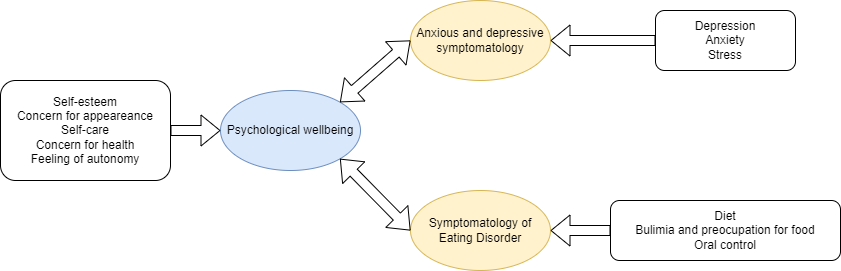
\includegraphics[scale=0.53]{img/introduction/vall_diagram.png}
    \caption{Relational model with the psychological impact of confinement to symptoms~\cite{vall2021impacto}.}
    \label{fig:vall_diagram}
\end{figure}


% ######################## NO SE HA METIDO ########################################
% -------------------Problemas que constan los TCAs --> nivel sanitario y sociologico -------------------
%EAT-26, EAT-40 y SCOFF --> instrumentos para medir frecuencias, chequear para dar numeros en este apartado
% ##################################################################################


% -------------------Social networks and eating disorders (check resources de anteproyecto) -------------------
%Articulo covid + tecnologia + enfermedades mentales: http://www.dspace.uce.edu.ec/handle/25000/25604
% NO USADO -  carta a director anorexia: https://www.scielo.cl/scielo.php?pid=S2452-60532022005000319&script=sci_arttext


This Master Thesis has been developed on the topic of Mental Health and the relationship of this with technology and social networks. The aim to know how the use of these impacts wellness. 

%After an exhaustive literature review, it has been determined that there is a significant association between inappropriate and prolonged use of social networks and the effects of mental health, finding mainly anxious, depressive, stressful and compulsive patterns among others. Therefore, they have determined that social networks can lead to public health problems~\cite{pozo2022impacto}.

The importance of Eating Disorders after the pandemic has been understood, especially in young women today. Technology and in particular social networks, as a means of communication and expression, play a decisive role in the well-being of current society and particularly in the development of disorders.

Making use of these social networks, large amounts of information can be extracted and subsequently analysed, processed and used to improve the most critical part of these Eating Disorders, detection. The proposed system in this project will be used to help people to detect and analyse profiles of users potentially suffering from a disorder, in order to speed up the clinical diagnosis process, which is a key factor to take into account when treating a patient with this type of problem.

For implementing this system, we will use text classification techniques for analysing data coming from social networks. The obtained results will be presented in an engaging user interface easy and quick to use for the user to get a prediction as soon as possible.

%\clearpage

\section{Project goals}
\label{sec:goals}
The goals of this Master Thesis have been defined from the beginning towards developing a social contribution that tackles one problem from the current society: Eating Disorders. With that in mind, the main goal of this project is to \textbf{develop a system for the analysis and detection of Eating Disorder-related mental health problems in social networks}. The application will integrate artificial intelligence technologies such as Natural Language Processing (NLP) and machine learning to detect these problems working with user data extracted from social media. The purpose of this tool is the \textbf{detection and analysis of user publications referring to Eating Behavior Disorders on social networks}. For this, several sub tasks are required:

\begin{itemize}
    \item Data collection, processing and analysis
    \item Design and implementation of machine learning models able to detect eating disorders from social media
    \item Training and evaluation the proposed models using the obtained datasets
    \item Development of a web application that integrates the proposed models for detecting and analyzing eating disorders
    \item System evaluation in a case study
    \item Integration of our system with a Task Automation Service (TAS) in order to enhance our system's features
\end{itemize}

\clearpage

\section{Structure of this document}

The remaining structure of this document is as follows.

\textbf{\textit{Chapter 2. State of art}}

In this chapter, we will focus on what is already known in different areas that are related to this Master Thesis. In addition, we will discuss the enabling technologies of
the project.

\textbf{\textit{Chapter 3. Eating Disorder detection}} 

In this chapter we will take a look on the Machine Learning techniques we have applied to get the necessary data to power the project. We will be explaining the data, the processing, the results and the validation we will implement and get from different models for taking a decision on what is better adjusted to our case.

\textbf{\textit{Chapter 4. Architecture}} 

In this chapter we will break down the design and the patterns followed for implementing the system we want to build in this project.

\textbf{\textit{Chapter 5. Case study}}

Here, the obtained results from the system will be presented for digging into what we have done.

\textbf{\textit{Chapter 6. Conclusions}} 

In this last chapter we will expose the conclusions taken from this Master Thesis and we will complete which are the future lines of work.

\chapter{State of Art}
\label{chap:state-of-art}
\textit{In this Chapter we will introduce the state of art of the project in relation with Eating Disorders and the work that has been done until now. Besides, we will discuss the technologies that enabled the realization of this project.}

\clearpage
\section{Mental illness: Eating Disorders}
Eating Disorders are a latent problem in today's society on which light needs to be shed. They are problems that historically have not had much importance, but in recent years the awareness in them has been increasing. In this section we will talk about Eating Disorders and what is known so far.

In order to situate this type of illness, it is necessary to first understand Mental Health and its implications, for which the Biopsychosocial model is presented. This model was created by Dr. George Engel and John Romano (1977), and it helps to have a broad picture of Mental health analysing and breaking down different aspects to take into account when tackling the topic. 

%MODEL OF MENTAL HEALTH ------------------------------------
% https://www.open.edu/openlearn/science-maths-technology/exploring-the-relationship-between-anxiety-and-depression/content-section-2
% 1 - INTERESTING BIOPSYCHOSOCIAL model for Mental Health: https://www.careershodh.com/what-is-biopsychosocial-model-of-health/
% BIOPSYCHOSOCIAL EDs: https://withinhealth.com/blog/posts/what-causes-an-eating-disorder-a-biopsychosocial-perspective
% https://www.researchgate.net/publication/8330681_Cognitive-Behavioral_Theories_of_Eating_Disorders

The framework considers biological, psychological and social aspects and their interactions to understand health, illness and health care delivery. This model is both a practical clinical guide and a philosophy of clinical care. The latter is concerned with understanding how suffering, disease and illness are affected from the molecular to the societal level. At the practical dimension, it is a way of looking at the subject's experience as a key element in human care, accurate diagnosis and health outcomes

As can be seen in Figure \ref{fig:biopsychosocial}, the aforementioned model has 3 distinct parts, the \textbf{biological}, which includes physiological pathologies; the \textbf{psychological}, under which fall emotions, thoughts and behaviours such as distress, fear, avoidance, etc.; and the \textbf{social}, which includes cultural, socio-economic and socio-environmental factors such as circumstances that the subject may experience at work or in the family.

\begin{figure}[!htp]
    \centering
    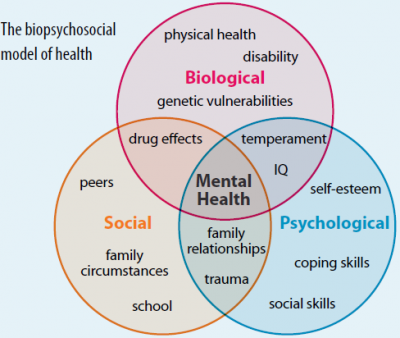
\includegraphics[scale=0.6]{img/state-of-art/biopsychosocial model.png}
    %\begin{minipage}{1}
    %\footnotesize
    %\emph{YOUR NOTES}
    %\end{minipage}
    \caption{Biopsychosocial Model of Health~\cite{Biopsych52:online}.}
    \label{fig:biopsychosocial}
\end{figure}

%ASSOCIATION WITH MODEL OF EDs------------------------------------
%\section{Model of mental illness and ED}
Coming back to the topic of interest, studies like~\cite{WhatCaus58:online} have particularised this Biopsychosocial model to Eating Disorders. In the Table~\ref{tab:biopsychosocialForEDs} we can find the aspects specified for each category.


\begin{table}[htp]
\begin{tabular}{|c|c|c|}
\hline
\textbf{Biological} & \textbf{Psychological} & \textbf{Social} \\ \hline
\begin{tabular}[c]{@{}c@{}}Family and personal history \\ of dieting and overeating\end{tabular} & Perfectionism & \begin{tabular}[c]{@{}c@{}}Weight-related teasing \\ and bullying\end{tabular} \\ \hline
High parental control & Novelty-seeking traits & \begin{tabular}[c]{@{}c@{}}Internalizing body image ideals \end{tabular} \\ \hline
\begin{tabular}[c]{@{}c@{}}Parental substance \\ use disorder\end{tabular} & Neuroticism & Separation from parent \\ \hline
\begin{tabular}[c]{@{}c@{}}Type I diabetes \\ (insulin-dependent)\end{tabular} & Conduct disorder & Weight stigma \\ \hline 
& Physical or sexual abuse & \begin{tabular}[c]{@{}c@{}}Acculturation, or assimilation \\ into Western culture\end{tabular} \\ \hline
& \begin{tabular}[c]{@{}c@{}}High levels of body \\ image dissatisfaction\end{tabular} & Intergenerational trauma\\ \hline
& \begin{tabular}[c]{@{}c@{}}Personal history of \\ an anxiety disorder\end{tabular} & \\ \hline
\end{tabular}
\caption{Biopsychosocial model for Eating Disorders.}
\label{tab:biopsychosocialForEDs}
\end{table}


These indicators potentially show, if present in a subject, the possible suffering of an Eating Disorder, although the final diagnosis must be made by a professional to confirm and start treatment. 

% TALK ABOUT METHODS TO DIAGNOSE EDs--------------------------------------------------------
% https://www.aafp.org/pubs/afp/issues/2003/0115/p297.html
%https://books.google.es/books?hl=es&lr=&id=mM7SAgAAQBAJ&oi=fnd&pg=PA155&dq=diagnosis+of+eating+disorder&ots=GA8hyKuevS&sig=sJShW_lqCcRK1S43G2mtpT-ihRg#v=onepage&q=diagnosis%20of%20eating%20disorder&f=false
% https://journals.sagepub.com/doi/abs/10.1177/070674379504000805

As experts have discussed~\cite{pritts2003diagnosis}, a number of problems can mask the disorder and should be considered before a diagnosis of an Eating Disorder is made, such as hyperthyroidism, malignancy, inflammatory bowel disease, immunodeficiency, malabsorption, chronic infections, Addison's disease and diabetes. A preoccupation with weight is observed in most patients with a health problem that leads to eating problems, but it is the patients who are diagnosed with an Eating Disorder who manifest a distortion of body image and want to be underweight.

The process of the medical diagnostic of the main three Eating Disorders (Anorexia Nervosa, Bulimia Nervosa and Binge Eating) needs to be emphasized. These diseases and their diagnostic are going to be tackled hereafter. According to the paper written by Garfinkel in 1995~\cite{garfinkel1995views}, several criteria for classifying and diagnosing Anorexia Nervosa, Bulimia Nervosa and Binge-Eating Disorder are defined.


\myparagraph{Anorexia Nervosa}
Following the scientific papers, Anorexia Nervosa is the \textit{``eating disorder, universally associated with emaciation and commonly accompanied by marked increases in physical activity''}~\cite{bulik2005anorexia}. The criteria for conducting the diagnosis this illness is defined as follows.
\begin{itemize}
    \item Refusal to maintain body weight at or above a minimally normal weight forage and height, e.g., weight loss leading to maintenance of body weight less than 85\% of that expected; or failure to make expected weight gain during a period of growth, leading to body weight less than 85\% of that expected.
    \item Intense fear of gaining weight or becoming fat, even though underweight.
    \item Disturbance in the way in which one's body weight or shape is experienced, denial of the seriousness of current low body weight, or undue influence of body shape and weight on self-evaluation.
    \item In post-menarcheal females amenorrhea, i.e., absence of at least 3 consecutive menstrual cycles. (A woman is considered to have amenorrhea if her periods occur only following hormone)
\end{itemize}

It has two sub types, which are i)Binge-Eating/Purging Type, in which the individuals have purging or binge-eating behaviour; ii) Restricting type, in which the subjects who suffer it limit calorie intake.


\myparagraph{Bulimia Nervosa}
This Eating Disorder is marked by episodes of binge eating followed by purging behaviors to prevent gain, as marked in the paper from Dr. Mehler~\cite{mehler2003bulimia}. In contrast to anorexia nervosa, which is characterized by a weight that is less than 85 percent of the normal value, most persons with bulimia are of normal weight. The criteria defined for diagnosis is defined in DSM-IV (Diagnostic and Statistical Manual)~\cite{widiger1997dsm} as follows.
\begin{itemize}
    \item Recurrent episodes of binge eating. An episode of binge eating is characterized by both of the following:
    \begin{itemize}
        \item Eating, in a discrete period of time (e.g., within any 2-hour period), an amount of food that is definitely larger than most people would eat during a similar period of time and under similar circumstances.
        \item A sense of lack of control over eating during the episode (e.g., a feeling that one cannot stop eating or control what or how much one is eating).
    \end{itemize}
    \item Recurrent inappropriate compensatory behaviour in order to prevent weight gain, such as: self-induced vomiting; misuse of laxatives, diuretics or other medications; fasting; or excessive exercise.
    \item The binge eating and inappropriate compensatory behaviours both occur, on average, at least twice a week for 3 months.
    \item Self-evaluation is unduly influenced by body shape and weight.
    \item The disturbance does not occur exclusively during episodes of anorexia nervosa.
\end{itemize}

As Anorexia Nervosa, it has also two sub types: i) Purging type, when the person has regularly in self-induced vomiting or the misuse of
laxatives, diuretics or enemas; ii)Nonpurging Type, when the patient is using inappropriate compensatory behaviours like fasting or exercise.

\myparagraph{Binge-Eating Disorder}
This disorder was a new introduction in the DSM-IV, although it is not a formal diagnosis within the DSM-IV, but in day-to-day clinical practice the diagnosis seems to be generally accepted. People with the BED-syndrome have binge eating episodes as do subjects with bulimia nervosa, but unlike the latter they do not engage in compensatory behaviours, according to what Dingemans states~\cite{dingemans2002binge}. The criteria to follow in order to diagnose it is as follows.
\begin{itemize}
    \item Recurrent episodes of binge eating. An episode of binge eating is characterized by both of the following:
    \begin{itemize}
        \item Eating, in a discrete period of time (e.c., within any 2-hour period), an amount of food that is definitely larger than most people would eat in a similar period of time under similar circumstances.
        \item Asense of lack of control over eating during the episode (e.g., a feeling that one cannot stop eating or control what or how much one is eating).
    \end{itemize}
    \item The binge-eating episodes are associated with 3 (or more) of the following:
    \begin{itemize}
        \item Eating much more rapidly than normal.
        \item Eating until feeling uncomfortably full.
        \item Eating large amounts of food when not feeling physically hungry.
        \item Eating alone because of being embarrassed by how much one is eating.
        \item Feeling disgusted with oneself, depressed or very guilty after overeating.
    \end{itemize}
    \item Marked distress regarding binge eating is present
    \item The binge eating occurs, on average, at least 2 days a week for 6 months.
    \item The binge eating is not associated with the regular use of inappropriate compensatory behaviours (e.g., purging, fasting, excessive exercise) and does not occur exclusively during the course of anorexia nervosa or bulimia nervosa.

\end{itemize}

With all of the above in mind, the aim of this project is to design and implement a system that will help diagnose these illnesses. This will serve as a complementary tool and as an orientation aid to the medical methods used today, because these are irreplaceable and also necessary in mental illnesses.




\section{Related work}
\label{sec:studies}

%https://dl.acm.org/doi/pdf/10.1145/3366030.3366058
%https://www.jmir.org/2015/11/e256/
% INTERESANTE COMPARACION BERT MODEL: https://medinform.jmir.org/2022/2/e34492/
A research has been conducted for gaining knowledge on the field and the already published documents. One study~\cite{oksanen2015pro}, which analysed videos and comments from YouTube channels related to pro-anorexia and anti-anorexia communities, was found. It comments that, although pro-anorexia videos are widespread on the platform, videos that promote help and oppose the community are more popular, having more positive comments and feedback. This makes anti-pro-anorexia communities into helping forces that professionals should give more support to.

Another scientific paper~\cite{benitez2022traditional} mentions other models which have also importance in the field. They are the so-called Bidirectional Encoder Representations from Transformer or also known as BERT models, which are discussed next. This study focused on finding Machine Learning models capable of efficiently categorising tweets about Eating Disorders, the main objective of our system.

For this purpose, tweets related to Eating Disorders were collected and a subset of 2000 tweets were classified into different categories that would help to better understand the collected material. Traditional and deep learning machine learning methods were used and then evaluated with accuracy, F1 score and computational time. 

Among the traditional methods, Random Forest was used, which will be discussed below, and, as reported in the paper, BERT models had the best score of all the techniques used, ranging from 71.1\% to 86.4\%, although they took the longest computation time. Methods such as Recurrent Neural Networks or Bidirectional long short-term memory were also used. These were scoring better than Random Forest but without reaching the accuracy of the BERT models.

% METER ALGUN PAPER MAS??? SOLO INCLUIDOS 2


This project will make use of all these knowledge and resources for embarking on the implementation of the application. But first, in order to start, a basic knowledge of the technologies that will shape the system is needed. Further explanations are detailed in the section below. 


\section{Enabling Technologies}
This Section will tackle the different technologies and techniques supporting this Master Thesis. The part of text classification, which includes all the Machine Learning mechanisms, and the part of the semantic task automation will be reviewed.


\subsection{Text Classification}
This Master Thesis is based on text classification methods. These techniques allow us to identify and extract information from existing resources using Machine Learning. Using them, we can determine what a person thinks about a particular topic, in our case Eating Disorders. This position can be a value judgement, a communication intention or an emotional state.

\subsubsection{Text Classification Techniques}

To understand the different problems of Text Classification it is important to review the architecture of this, as can be seen in Figure \ref{fig:text-clasification-architecture}, which will generally found in almost all text classification cases conducted today. It is divided into 5 parts described below:


\begin{itemize}
    \item Corpus: input of documents in any format (XML, JSON, CSV, PDF, etc.)
    \item Document processing: documents are preprocessed using linguistic tools like tokenization, part of speech tagging, lemmatization, stemming, etc.
    \item Lexicons and linguistic resources: supporters of the whole architecture
    \item Document analysis: key part where the documents that are preprocessed are interpreted using the linguistic resources
    \item Scores: presentation of the results after analysing documents, using visualization tools.
\end{itemize}


\begin{figure}[!htp]
    \centering
    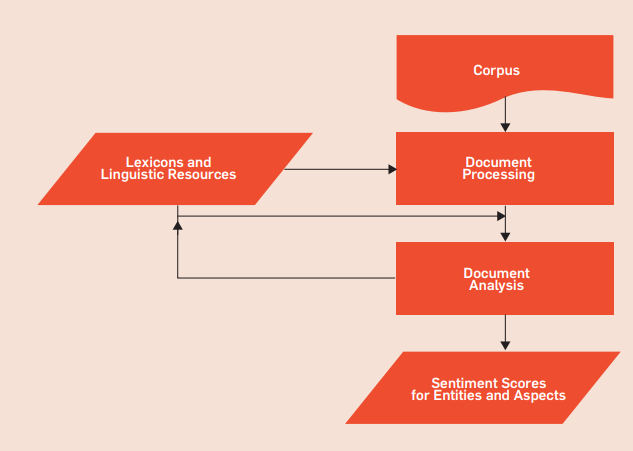
\includegraphics[scale=0.85]{img/state-of-art/text-classification-architecture.png}

    \caption{Generic text classification system architecture~\cite{feldman2013techniques}.}
    \label{fig:text-clasification-architecture}
\end{figure}

% TECNICAS DE ANALISIS DE SENTIMIENTOS ----------------------------------------
% https://dl.acm.org/doi/abs/10.1145/2436256.2436274?casa_token=lqpbt-cBaHYAAAAA:x2yhJourTm6uZJepBIzElTx3v759Iv2UVKWlQi1CJJEsUy1qxoJfzYHWRs6XGJy9onXToAkI-Ow2kg

Knowing this architecture, there are some problems to solve while performing the text classification that the expert have spotted as key for the success of the learning~\cite{feldman2013techniques}. There are different ways of approaching a problem of analysis such as this Master Thesis, generating different approaches that must be know before digging into the technical part. The problems of document-level classification, sentence-level classification and lexicon acquisition will be discussed.

\myparagraph{Document-level classification}
This form is the simplest of all text classification, which assumes that the document itself has a value judgement on a main subject expressed by the author of the subject. This approach can be tackled with both supervised and unsupervised learning. The first one takes the assumption that there is a finite set of classes(e.g. the simplest case, positive and negative) into which the document must be classified having training data for each one. The unsupervised approach is based on determining the semantic orientation (SO) of certain phrases in the document.

Researchers have found good results when each document is represented as a simple bag of words, meanwhile the unsupervised approach has worked well in English but it is lacking linguistic resources when switching to other major spoken languages such as Chinese and Spanish and thus, throwing worse results.

\myparagraph{Sentence-level classification}
This approach is considering that a document can contain different opinions about the same subjects, so when we need to have a deeper zoom for analyse it and move to the sentence level this it the approach that is more adequate. It consist in assuming that each sentence has a different opinion, and then it can be relaxed analysing different phrases and collect them into groups for then apply the machine learning techniques.

%\myparagraph{Aspect-based classification}
%Aspect-based classification opens the spectrum of entities to which the analysis is done. While the previous two work when the author refers to one entity, in many cases the people talk about different attributes that need to be consider since the opinion about them can be different. This approach is defined as \textit{``research problem that focuses on the recognition of all expressions within a given document and the aspects to which they refer''}.

%There are two ways of handling kind of analysis, the classical approach of this is extracting all noun phrases (NPs) and keep the ones whose frequency is higher an experimentally determined threshold, and the other one is use a phrase dependency parser that uses known expressions to search for additional aspects.

%\myparagraph{Comparative classification}
%Usually the authors provide their opinion about a subject through the comparison with other subjects so the goal of this technique is to assess which sentence contains a comparative opinion and extract the preferred entities in each. Researchers in this field have found the most common words that we use for the 98\% of the cases so with them we can start separating the comparison and analyse them properly~\cite{jindal2006identifying}.

\myparagraph{Lexicon Acquisition}
This part is usually the most crucial resource for the text classification algorithms and there are three ways to acquire it: i) manually, in which people code the lexicon by hand; ii) dictionary-based approaches in which with seed words the lexicon is expanded using external resources; iii) corpus-based approaches where a set of seed words the lexicon is expanded by using a large corpus of documents.\\

\subsubsection{Machine Learning}
As mentioned before, text classification is based on machine learning, which has different definitions, the first being the one provided by Arthur Samuel in 1959 which defines this concept as \textit{``Field of study that gives computers the ability to learn without being explicitly programmed''}~\cite{samuel1959some}.
Over the years it has undergone a great evolution, having a newest definition like the one written in~\cite{el2015machine}: \textit{``Machine learning is an evolving branch of computational algorithms that are designed to emulate human intelligence by learning from the surrounding environment''}.

There are different techniques encompassed within Machine Learning in order to better adapt to the use case study on each occasion. T.Ayodele recounts that there are specifically six types~\cite{ayodele2010types}: Supervised Learning, Unsupervised Learning, Semi-supervised Learning,  Reinforcement Learning, Transduction and Learning to learn, but this Master Thesis will focus on the most relevant ones which are Supervised , Unsupervised and Reinforcement Learning.
\myparagraph{Supervised Learning}
Method used commonly in classification problems since the principal goal is to the computer to learn a classification system that we have already created. In general, this type of learning is optimal for any problem where a classification of elements is needed and it is easy to define. 

These desired classification could be for both discrete(\textit{e.g.} an integer, a label or a boolean) and continues values, and each case it can be called as \textit{Classification} or \textit{Regressive} problems, and the two of them are tackled in a similar way. In the Figure \ref{fig:supervised-learning} we can see an example for better understanding the difference among the described types.

\begin{figure}[!h]
    \centering
    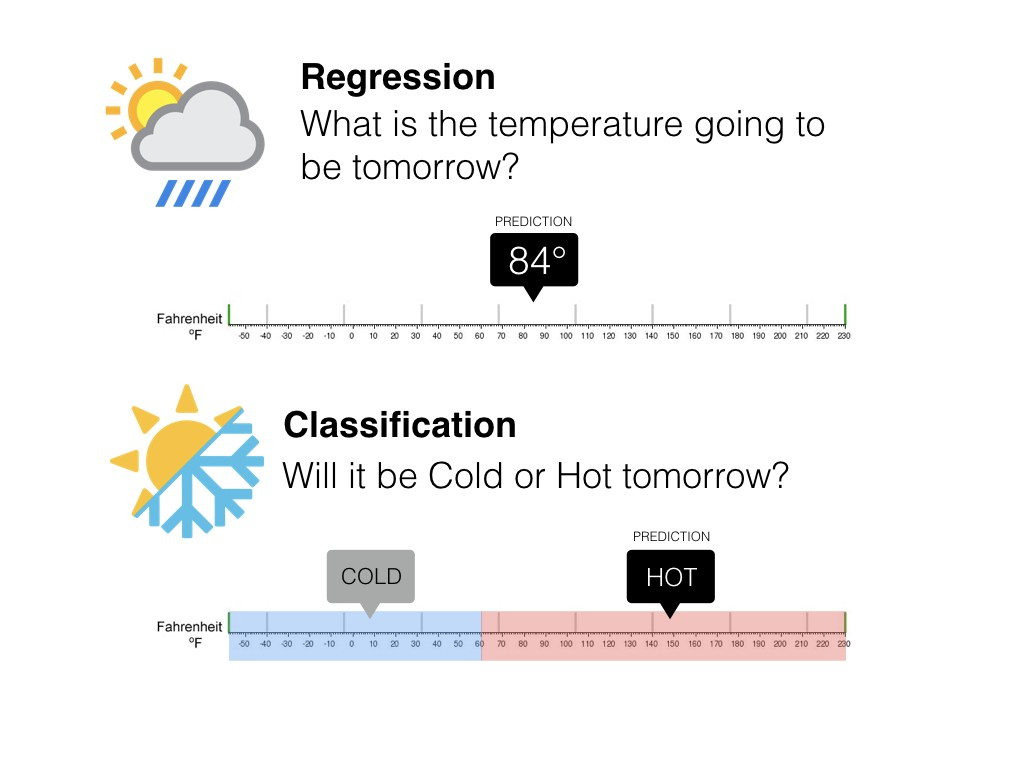
\includegraphics[scale=0.27]{img/state-of-art/supervised-learning.jpeg}
    \caption{Different types of Supervised Learning.}
    \label{fig:supervised-learning}
\end{figure}

Supervised Learning is the most common technique in Neural Networks and Decision Trees, since these are highly dependent on the information provided by already determined classifications.
%% SE PODRIA EXTENDER SUPERVISED LEARNING

\myparagraph{Unsupervised Learning}
This type of learning aims to induce patterns in the observed data without having any knowledge about them, which makes the task much more complicated \textit{a priori}. The most commonly used technique in this case is clustering, which is a data mining technique that groups elements by similarities and induces classifications. These algorithms are used to process unclassified objects into information structures. There are several types of clustering, such as exclusive, overlapping, hierarchical, and probabilistic clustering~\cite{WhatisUn52:online}.

%% HABLAR DE DIMENSIONALITY REDUCTION???

An example of an unsupervised algorithm is the so-called k-means clustering, which aims at partitioning a set of n observations into k groups, where each observation belongs to the group whose mean value is closer to the nearest.
\myparagraph{Reinforcement Learning}
One of the most important types of learning is Reinforcement Learning, which is defined in~\cite{sutton2018reinforcement} as follows: ``\textit{Reinforcement learning is learning what to do-how to map situations to actions-so as to maximize a numerical reward signal''.}  The actions to take are not told, but instead, the learner must discover which actions serve the most reward.

This learning is rather empirical, in that each decision intelligence makes is evaluated and rewarded positively or negatively depending on the success of that decision. This is why it often takes many attempts to bring the learning to the desired accuracy.\\

Now that the basics have been understood and the different paths that can be taken using Machine Learning have been explained, the models with the highest relevance for the Machine Learning part of this project are going to be discussed.

\subsubsection{Machine Learning models}
An important part of this project is the used model for making the prediction. A research and an analysis have been performed for getting more knowledge on the tools that are available for reaching this Master Thesis' objective.

Before starting, it is important to mark the kinds of the algorithms that have been checked. One type of them are the algorithms that have been used for some time now that are designated in this project as `Traditional Models' which include the Random Forest, SVM and Logistic Regression; and the BERT models which are pretrained models that adapt to the available data and are based on Neural Networks.

In this subsection this models are going to be investigated for getting more information on them and their functioning.

\myparagraph{Traditional Models}
For this project, as mentioned, traditional models are those that have not been pre-trained and are historically more consolidated in the field of Machine Learning and Artificial Intelligence, despite this being a relatively new and booming field.

\mysubparagraph{Random Forest}
Random Forest~\cite{breiman2001random} is a decision tree-based Machine Learning algorithm used for classification or regression of data by constructing many decision trees when training the model. These models are sampled independently and with the same distribution for all the members. In the case of classification, the output tree is the class selected by the largest number of trees, as in our case. A representation of it can be seen in the Figure~\ref{fig:random-forest}.

\begin{figure}[!htp]
    \centering
    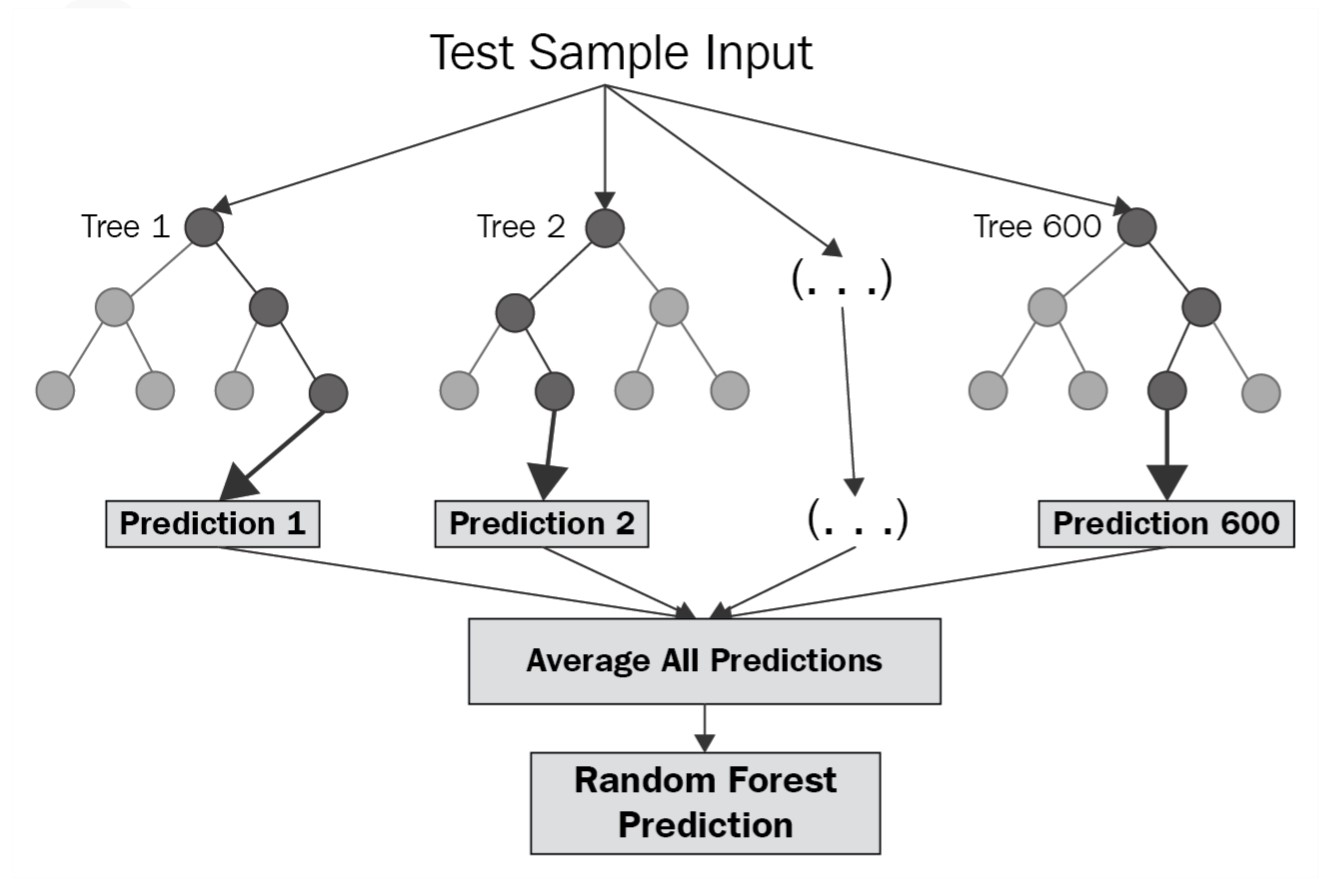
\includegraphics[scale=0.28]{img/detection/random-forest.jpg}
    \caption{Random Forest model representation.}
    \label{fig:random-forest}
\end{figure}

The generalization error for these models converges to a limit with the increase of the size of the forest itself. This error depends on the strength of the singular trees and the correlation among them. This algorithm corrects the flaw in decision trees of overfitting the training set, \textit{i.e.} overtraining a learning algorithm so much that it is only effective under very specific conditions, those of the training data.

\mysubparagraph{SVM}
The Support Vector Machine algorithm~\cite{chauhan2019problem}, also known as SVM, is an optimal margin based classification technique in Machine Learning. The objective of this is to find a hyperplane that best separates two different classes of data points,\textit{ i.e.} with the widest margin between the two classes. 

It is a binary linear classifier which has been enhanced to support non-linear data using various Kernels. SVM is continuously improving since its invention and the experts have pose different formulations for solving SVM. 

\begin{figure}[!htp]
    \centering
    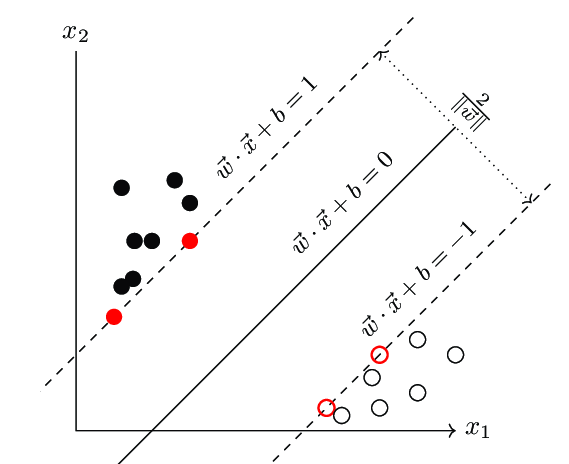
\includegraphics[scale=0.37]{img/detection/SVM.png}
    \caption{SVM model representation.}
    \label{fig:SVM}
\end{figure}

The margin raised before is defined as the maximum width of the region parallel to this hyperplane that has no interior data points. This algorithm only works on problems that allow linear separation, maximising the aforementioned margin as it can be seen in Figure~\ref{fig:SVM}.

\mysubparagraph{Logistic Regression}
Logistic regression is one of the most important statistical and data mining techniques for analysis and classification for datasets that are binary and proportional~\cite{maalouf2011logistic}. This model is within supervised learning and is used to predict the categorical dependent variable given a set of independent variables. This predicted output can take both categorical and discrete values and is used for classification problems. In this regression, an attempt is made to fit the values within an ``S" shaped logistic function that predicts between two maximum values, either 0 or 1 as can be seen in Figure~\ref{fig:LogisticRegression}.

\begin{figure}[!htp]
    \centering
    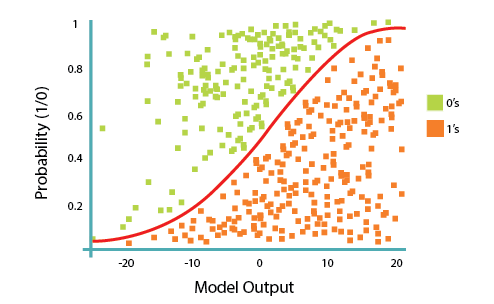
\includegraphics[scale=0.6]{img/detection/LogisticRegression.png}
    \caption{Logistic Regression representation model.}
    \label{fig:LogisticRegression}
\end{figure}



\myparagraph{BERT Models}
%% METER ARQUITECTURA MODELS

After explaining the traditional models, BERT or Bidirectional Encoder Representations from Transformers are going to be explained. 

BERT models~\cite{acheampong2021transformer} are pre-trained and open source machine learning techniques based on neural networks for NLP developed by Google in 2018. These algorithms have been used in the company's search engine since 2019. BERT makes use of Transformer, an attention mechanism that learns the contextual relationships between words and includes two different mechanisms, an encoder that reads the input text and a decoder that produces a prediction. This encoder is the necessary element, because BERT's goal is to generate a language model.

BERT models can be used for a number of different linguistic tasks by adding only a small layer to the core model. In classification tasks, as is the case in this project and in sentiment analysis, they are performed in a similar way to Next Sentence Prediction (NSP) techniques, by adding a classification layer on top of the output of the token transformer (CLS)~\cite{BERTExpl89:online}.

In the NSP training process, the model is provided with pairs of sentences as input and learns whether the second sentence of the pair is the next sentence in the original document to learn about the context. 50\% of the input sentence pairs are the subsequent sentences in the original document and the other 50\% are randomly chosen and disconnected sentences. In order to process the input text the following steps are needed to be performed, as it can be seen in Figure~\ref{fig:BERTinput}.

\begin{enumerate}
    \item A CLS token and a SEP token are inserted at the beginning and end of each sentence respectively.
    \item A phrase embedding indicating phrase A or phrase B is added to each token.
    \item A positional inlay is added to each token to indicate its position in the sequence.
\end{enumerate}

\begin{figure}[!htp]
    \centering
    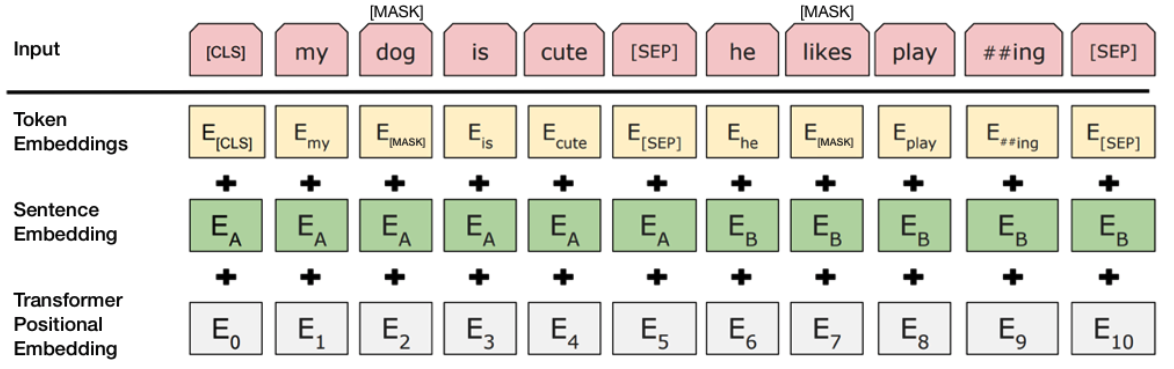
\includegraphics[scale=0.35]{img/detection/BERTinput.png}
    \caption{BERT input processing in NSP.}
    \label{fig:BERTinput}
\end{figure}
Once the input text has been pre-processed, to make the prediction of the second sentence over the first, the following is needed.

\begin{enumerate}
    \item Introducing the sequence to the Transformer model.
    \item The output of the [CLS] token is transformed into a 2x1 vector using one of classification.
    \item Calculate the probability with softmax or normalised exponential function.
\end{enumerate}

BERT models have also variants which provide different approaches optimised for specific use cases. In the project, models like roBERTa and concretely Mental roBERTa, which seeks to optimize BERT in various methodological parameters have been analysed. This model is focused on mental health problems and it helps to investigate hyperparameters such as larger pre-training datasets, batch sizes or text encoding.

A remark should be put as well on mBERT, a model which is based on BERT trained with a big corpus that support a large amount of languages. \\


% Parte de enabling technologies con python y modelos???
\subsubsection{Machine Learning Technologies}
For landing this project, decisions had to be made about the technologies to be used to implement the different blocks of the system. Different tools were chosen to implement it which are Python and its libraries for the Machine Learning part, Python Flask for the web server and Flutter for the user interface.

Python is a language that supports the development of Machine Learning very well with its pre-established libraries. It comes with many models already implemented, which are very easy to implement using of Jupiter Notebooks, a framework for interactive computation.

\myparagraph{Python and extensions}
Python~\cite{Welcomet44:online} is a programming language created in the late 1980s by Guido van Rossum at the Centre for Mathematics and Informatics (CWI, Centrum Wiskunde \& Informatica) in the Netherlands as a descendant of the ABC programming language. As a curiosity, the name language comes from its creator's fondness for the British comedians Monty Python. It is a high-level interpreted language whose focus is on the readability of the code, as well as being a multi-paradigm language (it partially supports object-oriented, imperative programming and to a lesser extent functional programming). It is a dynamic(a variable can take on values of different types), cross-platform and interpreted language, as the code is translated and executed at the same time.

In Python there are many open libraries that can be used for many different purposes, but we will focus on the one related to data mining and machine learning. For this purpose, there are libraries that implement data processing methods and models such as pandas, NTLK or sklearn, which we will detail below.

\mysubparagraph{Pandas}
Pandas~\cite{pandasPy20:online} is a Python library used in data science and computer science, developed as an extension of Numpy (another library that allows the use of vectors and matrices of various dimensions, as well as complex mathematical functions) for data management and analysis. It provides the ability to work with data structures and operate with this data, being this library a free and open software.

\mysubparagraph{NTLK}
Natural Language Toolkit~\cite{NLTKNatu6:online} (or NTLK) is a set of libraries for symbolic and statistical natural language processing, intended to support research in Natural Language Processing (NLP) or closely related areas such as empirical linguistics, artificial intelligence, cognitive science, machine learning and information retrieval, used as a tool and platform for prototyping and building research systems - it provides over fifty corpora and lexical resources, along with a suite of text processing tools for classification, tokenization, stemming, parsing and semantic reasoning.

\mysubparagraph{Sklearn}
Sklearn~\cite{scikitle66:online} is an open source library that includes several types of classification, regression and cluster analysis algorithms, designed to work together with NumPy or SciPy (another library of mathematical tools and algorithms). Algorithms such as SVM, Random Forest, K-means, etc. are implemented in it.


\subsection{Server framework}
In the part designed as a server, a study was made of the technologies available for its implementation and it was decided to use the Flask framework for Python due to the previous experience in the Bachelor Thesis that the author already had and the ease of implementation of this technology.

\myparagraph{Python Flask}
Flask~\cite{Welcomet8:online} is a micro web framework written in Python by Armin Ronacher of Pocoo, described as a microframework because of its minimalistic approach, requiring no particular libraries or tools. It does not add any integration with third-party components but common functions, although it does support the integration of extensions to add new functionalities such as form validation, upload handling, open authentication technologies, etc. An example of applications that use this framework are Pinterest and LinkedIn.


\subsection{App development}
To develop the application the future potential of the system was taken into accound and the decision of opting for a modular and multiplatform integration was taken. That is the reason why Flutter has its place in the project, which will be described next.

\myparagraph{Flutter}
Flutter~\cite{FlutterB22:online} is an open source SDK created by Google for application development, commonly used to develop user interfaces for web, Android and iOS, as well as the primary method for creating applications for Google Fuchsia. It was first known as ``Sky'' and was introduced on Android operating systems, having its first release in 2015 at the Dart developer summit and Preview 2 released at Google Developer Days in September 2018, until December 4 of that same year when the first version was released.

It is programmed in Dart, an open programming language also developed by Google, offering a modern alternative to javascript, whose philosophy is defined by one of its engineers as a \textit{``structured but flexible language for web programming''}.\\


The fundamentals of Machine Learning together with models and technologies have been reviewed, now in this Thesis we will talk about how do the project tackles and resolves the encountered problems. 

\subsection{Semantic Task Automation}

Semantic task automation will be used in this project as we mentioned in Section~\ref{sec:goals}. Using it, the project aims to provide user features for enhancing our system and provide it with different functionalities. The outcomes are going to be described here.

\subsubsection{Task Automation Services}
% https://www.gsi.upm.es/ontologies/ewe/ pillar de aqui estructura
Nowadays, automation is found in almost every task we perform, so much so that we are even unable to recognise that automation. This automations have also spread to the Web field, raising the need to be able to orchestrate and centralise them. Hence the need to create TAS or Task Automation Services~\cite{7155422}.

These Task Automation is a area which is increasing rapidly in these times and Task Automation Service provide a friendly user interface. They can be presented in really different ways, such as websites or as mobile apps\footnote{Some of the most popular services are called: ifttt, Zapier, CouldWork, Onx, Atooma or AutomateIt.}, where non-technical users can create their own automations in them. These automations take the form of Event-Condition-Action in which some actions are executed when a trigger happens. 

One interesting branch that is part of Semantic Web which is being investigated~\cite{electronics9081194} is the Task Automation Services using semantic techniques. This allows to have a standard data schema designed to adapt to a lot of use cases. In this context, we have analysed and researched on Evented WEb ontology (EWE) because is the technology on which our platform, which is described in the following.

\subsubsection{EWE}
% EWE MAIN ENTITIES  DIAGRAM
Evented WEb ontology or EWE~\cite{EWEOntol89:online} is an ontology which aims to enable the publishing of raw data from TAS, enable rule interoperability and provide a base vocabulary for building specific vocabularies for domains like Twitter Task Ontology or Evernote Task Ontology.

The diagram that represents EWE and its main concepts is the one that can be found in Figure~\ref{fig:ewediagram}. On it we can find the four cores of the ontology which are: Channel, Action, Event and Rule. 

\begin{figure}[!htp]
    \centering
    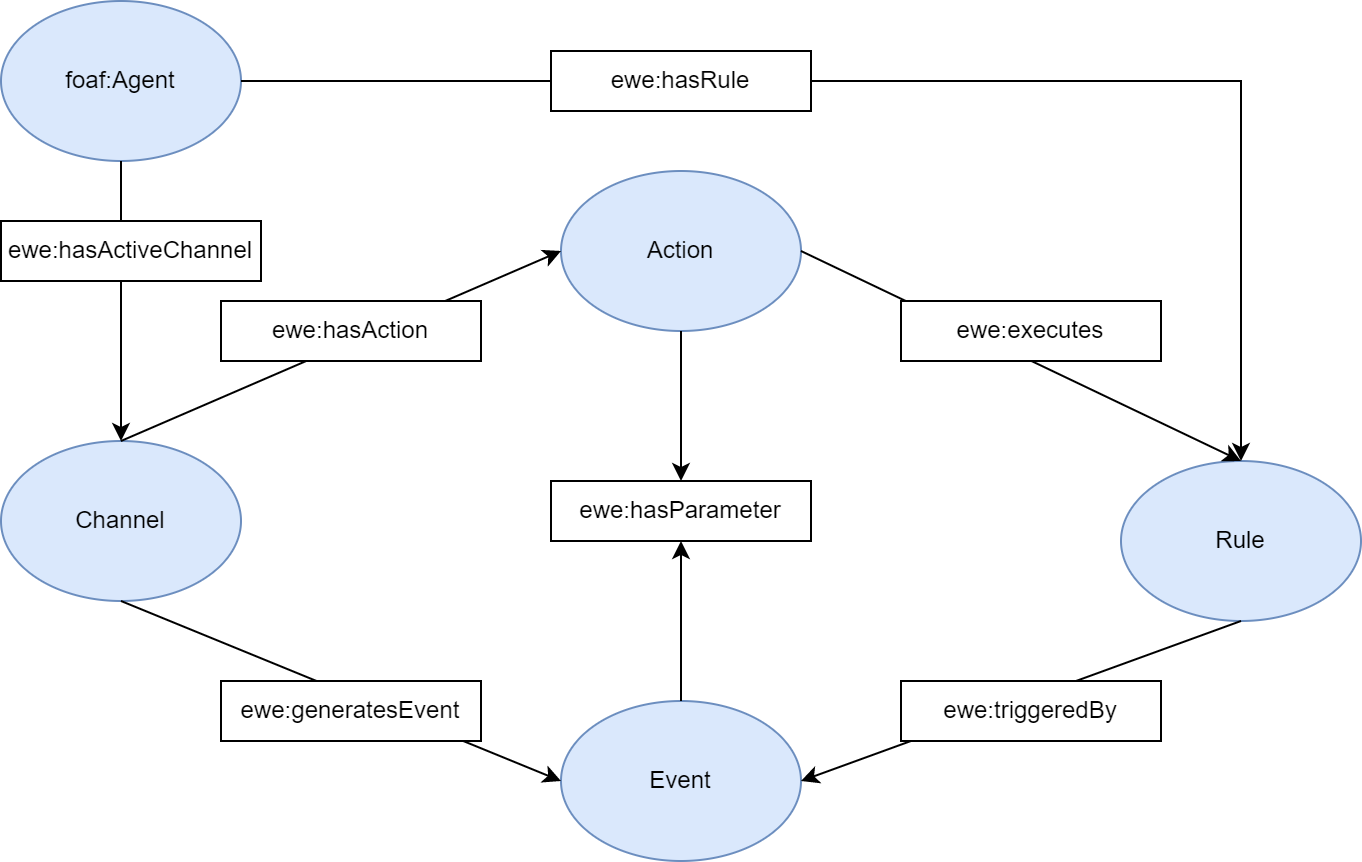
\includegraphics[scale=0.28]{img/state-of-art/EWEdiagram.png}
    \caption{Diagram of EWE entities and its relations.}
    \label{fig:ewediagram}
\end{figure}

This diagram has two kinds of entities, which are the classes, marked with circular figures in blue, and the relations among them, marked with with rectangles. Summarizing what these cores are for, the following list is presented.

\begin{itemize}
    \item The class \textit{Channel} defines an individual that can generate events, execute actions or can perform both.
    \item The class \textit{Event} is a particular occurrence in the process, and allows users to define the \textit{Rules} based on them.
    \item The class \textit{Action} defines the execution that can be taken after a certain \textit{Channel} triggers an \textit{Event}.
    \item The \textit{Rule} is the one defined the ECA model described before, in which a user can select which \textit{Channel} triggers which event that is landed executing a certain \textit{Action}.
\end{itemize}
There is an additional class designated as \textit{foaf:Agent} that is implemented under the EWE cores which check if there are \textit{Rules} for an active\textit{ Channel}.




\chapter{Eating Disorder detection}
% deteccion trastornos mentales : dataset, modelos y validacion de los modeloos (resultados)
\label{chap:architecture}
\textit{This chapter presents the methodology used in this work. It describes the overall architecture of the project, with the connections between the different components involved on the development of the project.}

\clearpage
\section{Machine Learning approach}
In order to design the solution we have taken into account the different perspectives that the project could take. To do so, we have decided to first experiment with labelled data in order to perform supervised learning and if we do not achieve good results, we would use other unsupervised learning techniques, as their implementation is much less trivial. In this chapter we are going to talk about the data we have used for this project and the results obtained by using them in Machine Learning models.

In addition, processing has been applied to this information, as we needed to optimise the input of the models so that it would take as much data as possible to make the prediction, which we will also talk about here, the procedures carried out with this data.

Furthermore, the data we are going to analyse are non-numerical, so we will adopt models that use such data and not numbers, a factor that we have had to take into account when selecting learning models. We have mainly focused on the traditional Random Forest, Logistic Regression and SVM models and other more complex pre-trained models such as BERT, specifically using BERT, Mental roBERTa and mBERT.


\subsection{Dataset}
\label{sec:dataset}
% https://arxiv.org/abs/1806.05258
% paper del que se saco
In order to train, validate and then classify and predict, we needed data related to the case study. For this purpose, a search for labelled datasets was made, in which several labelled datasets related to mental illnesses have been found. We decided to use the one introduced in~\cite{https://doi.org/10.48550/arxiv.1806.05258} which investigates the creation of high-precision patterns to identify diagnoses of nine mental illnesses and obtains labeled data without having to manually label it.

The dataset was published in conjunction with the paper, which is called SMHD and is a dataset of social media posts from users with different mental health conditions, including schizophrenia, bipolar disorder, depression, anxiety, obsessive-compulsive disorder, eating disorder, post-traumatic disorder, autism and attention-deficit disorder. In this project we have filtered the data related to Eating Disorders in order to focus on the topic of interest.


% estructura de los datos

In order to be able to go deeper into the data to be able to use them correctly, an analysis of the information present in the SMHD dataset taken has been carried out, in order to subsequently adapt the data to ingest them into the Machine Learning model. To do this, the type of data and its content have been determined in order to decide which are useful and which can be discarded. Subsequently, all this information will be processed in order to adapt it to our use case, in which we want to predict whether a person suffers from Eating Disorder or not by what they write. It should also be noted that, being linguistic and the data being in English, the models have been adjusted to that language, although explorations have been made with other models, as we will discuss in the Section~\ref{sec:models}.

This dataset consists of a set of Reddit posts, concretely 76203 entries of 331 users, labeled with binary classification for suffering an Eating Disorder. The binary label mean of the dataset is 0.345065, that means that around 34.5\% of the post are classified as positive and has an average of 161.13 words per posts, being the maximum a post of 12388 words. This is an strange case because the standard deviation is of 282.8 which indicates that posts are closer to the average number and the maximum number of words of the biggest post is an anomaly. In the Figure~\ref{fig:SMHDwordcloud} the most common used words are displayed.

\begin{figure}[!htp]
    \centering
    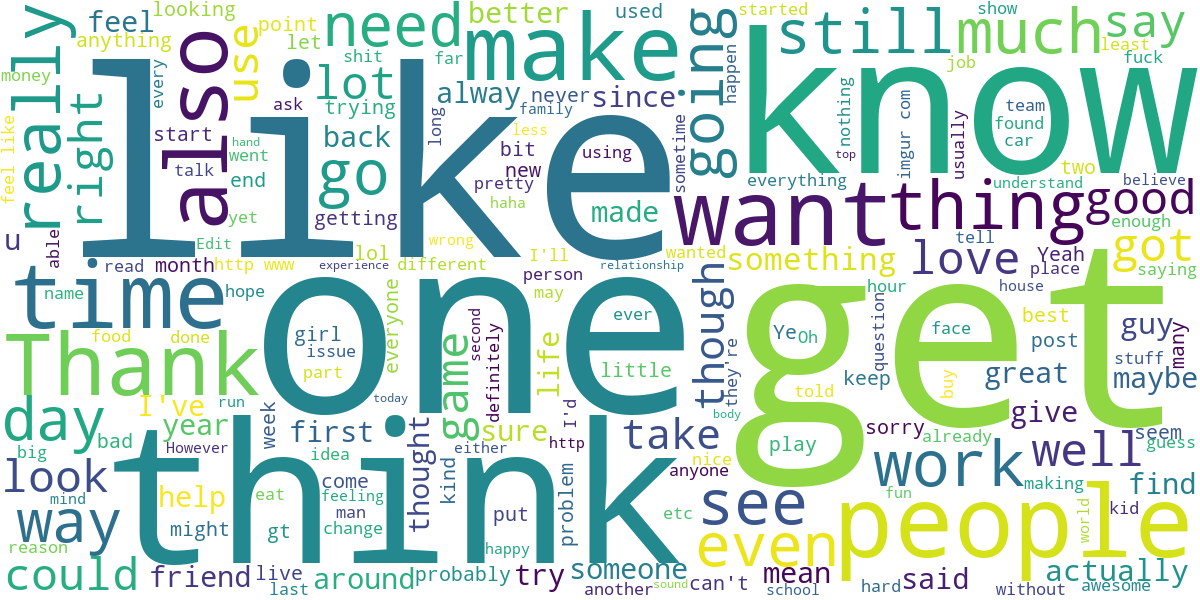
\includegraphics[scale=0.35]{img/detection/SMHD_wordcloud.png}
    \caption{Wordcloud of most common words in SMHD}
    \label{fig:SMHDwordcloud}
\end{figure}


% AQUI O EN CASE STUDY?
\subsection{Twitter Data}
As mentioned above, the aim of this project was to classify posts on social networks, in which we are going to focus mainly on Twitter. To do this, the data used will be tweets from the profile of the person to be analysed, which will then be passed through the Machine Learning algorithm to make the prediction, which is already trained and adapted to the data with the previously mentioned SMHD dataset.

% Scrapping de tweets
To do this, we need to get access to a Twitter API which takes information from the social network via a query. For this, we have used the tool snscrape~\cite{JustAnot83:online}, which allows us to take information from the tweets made by the person to be analysed. It is a Python package that can be easily installed using the pip manager, which allows us to take as many tweets as we want from a profile and put them in a text file in JSON format, as it can be seen in the code block described in Appendix~\ref{appendix:JSONsnscrape}.

% procesamiento de los textos
% recogida de mas datos: pic, username

As you can see in that Appendix, we have a lot of information in addition to what we need for our project, so we have to process the data and keep the ones we are really interested in. For this purpose, a processing method has been implemented within the developed server, which we will discuss in Chapter~\ref{chap:architecture}. In that Chapter we will discuss how we will use other data, as there are also other elements that can be useful for serving them in the application for making it more user-friendly. We are going take this parameters into account for elaborating the API response from our server.

\section{Preprocessing}
Once we had obtained the dataset with which we were going to do the training, we connected to a development environment in order to carry out the pre-processing. We have used the platform of the Jupiter Notebooks department and the Google Collab platform, both of which allow us to create notebooks in which to execute code, specifically Python code, and to have a virtual environment in which to do so.

We load the dataset using Pandas library in the development platform, which allows us to study in depth the characteristics of these as indicated in the Section~ref{sec:dataset} for the information of the SMHD dataset. We can extract different metrics from it, but what we are most interested in is to process the text to put it as input to the model, as it does not work with raw test, but we have to clean it and convert it.

In the Code~\ref{code:preprocessing} we see the treatment given to all the text in the dataset, in which we can see several processes that we are going to explain below.

\begin{lstlisting}[language=Python, caption={Preprocessing used function}, label={code:preprocessing}]
def preprocess(words):
    tokens = nltk.word_tokenize(words)
    porter = nltk.PorterStemmer()
    lemmas = [porter.stem(t) for t in tokens]
    stoplist = stopwords.words("english")
    lemmas_clean = [w for w in tokens if w not in stoplist]
    punctuation = set(string.punctuation)
    words = [w for w in lemmas_clean if  w not in punctuation]
    return words
\end{lstlisting}

\myparagraph{Tokenization}
Tokenization is a process used to change the text and separate the words of a sentence into an array of words separated by a comma, so that the model understands the input we are providing. For serving this purpose, as seen in the code mentioned above, the word\_tokenize method of the NTLK package has been used.

\myparagraph{Stemmization}
Stemmization is a technique whose aim is to reduce a word to its root or base unit, not necessarily a dictionary-based morphological root, but a part equal to or smaller than the word itself. These are typically rule-based algorithms, which can be seen as a heuristic process that cuts off the end of words. In this, a word is taken through a series of conditionals that determine how to cut it.

An example of this might be English suffixes such as "-ed" or "-ing" which do not have much linguistic relevance, being able to relate the words "play", "playing" and "played" which have the same root which is "play."

The stemming algorithm used in this case is Porter's, which is an algorithm from the 1980s whose aim is to erase the common endings of words so that they can be reduced to a common form. It is not very complex and its development is frozen. It is a good algorithm to start introducing in research branches, as it ensures reproducibility, but it is not recommended for use in a complex application due to its limitations.

\myparagraph{Punctuation and stopwords cleaning}
In order to clean the text, we need to eliminate the part of it that doesn't have any linguistic value like punctuation marks(\textit{e.g.} '.','!','?', etc) or stopwords (words, in general adverbs, prepositions, conjunctions and articles, that are meaningless \textit{e.g.} "the", "a", "an", etc.) among others, so we increase the relevance of the remaining items. In order to do so, we take the stopwords provided with the NTLK package and we search for occurences in our text for removing them afterwards.\\


After applying these techniques, we can proceed to pass the data and train the models to fit our data. In the following Section, we will discuss this topic.

\section{Used models}
As explained in the previous Section~\ref{sec:studies}, both traditional and newer machine learning methods have been employed. In this section we will look at what they consist of, the techniques used and the statistical results obtained.

In addition, in each model we will analyse the results obtained with them in order to evaluate the optimisation that they may have. To do this, it is necessary to know some statistical measurements that are going to be explained here but before that, we need to understand the basic concepts for making these statistics, which are the possible results from a prediction.
\begin{itemize}
    \item\textbf{ True positive (TP).} True positive is a result that has been predicted as positive and it is correctly predicted.
    \item\textbf{ False positive (FP).} False positive is a result that has been predicted as positive but it is incorrect, it should have been negative. 
    \item \textbf{True negative (TN).} True negative is a result that has been predicted as negative and it is correctly predicted. 
    \item \textbf{False negative (FN).} False negative is a result that has been predicted as negative but it is incorrect, it should have been positive.
\end{itemize}

With these concepts explained, we can dig into the concepts introduced before that we will use for evaluation of the models which are precision, recall, accuracy or F1-score.

\begin{itemize}
    \item \textbf{Precision.} Precision is defined as the number of true positives that have been among all the positive predictions. In an equation it would look like the following.
    \begin{equation}
        precision = \frac{TP}{TP + FP} 
    \end{equation}
    \item \textbf{Recall.} Recall is the measurement of the capacity of the model for classifying true positives.
    \begin{equation}
        recall = \frac{TP}{TP + FN} 
    \end{equation}
    \item \textbf{Accuracy.} Accuracy is the measure of the correct predictions that have been made.
    \begin{equation}
        accuracy = \frac{TP + TN}{TP + FP + TN + FN} 
    \end{equation}
    \item \textbf{F1-score.} F1-score is the mean of precision and recall
    \begin{equation}
        F1-score = \frac{2 * precision * recall}{precision + recall} 
    \end{equation}
    
\end{itemize}

\label{sec:models}
\subsection{Traditional Models}
In this project, we call traditional models those models that have not been pre-trained and are historically more consolidated in the field of Machine Learning and Artificial Intelligence, despite this being a relatively new and booming field.

\subsubsection{Random Forest}
Random Forest is a decision tree-based Machine Learning algorithm used for classification or regression of data by constructing many decision trees when training the model. In the case of classification, the output tree is the class selected by the largest number of trees, as in our case. A representation of it can be seen in the Figure~\ref{fig:random-forest}.

\begin{figure}[!htp]
    \centering
    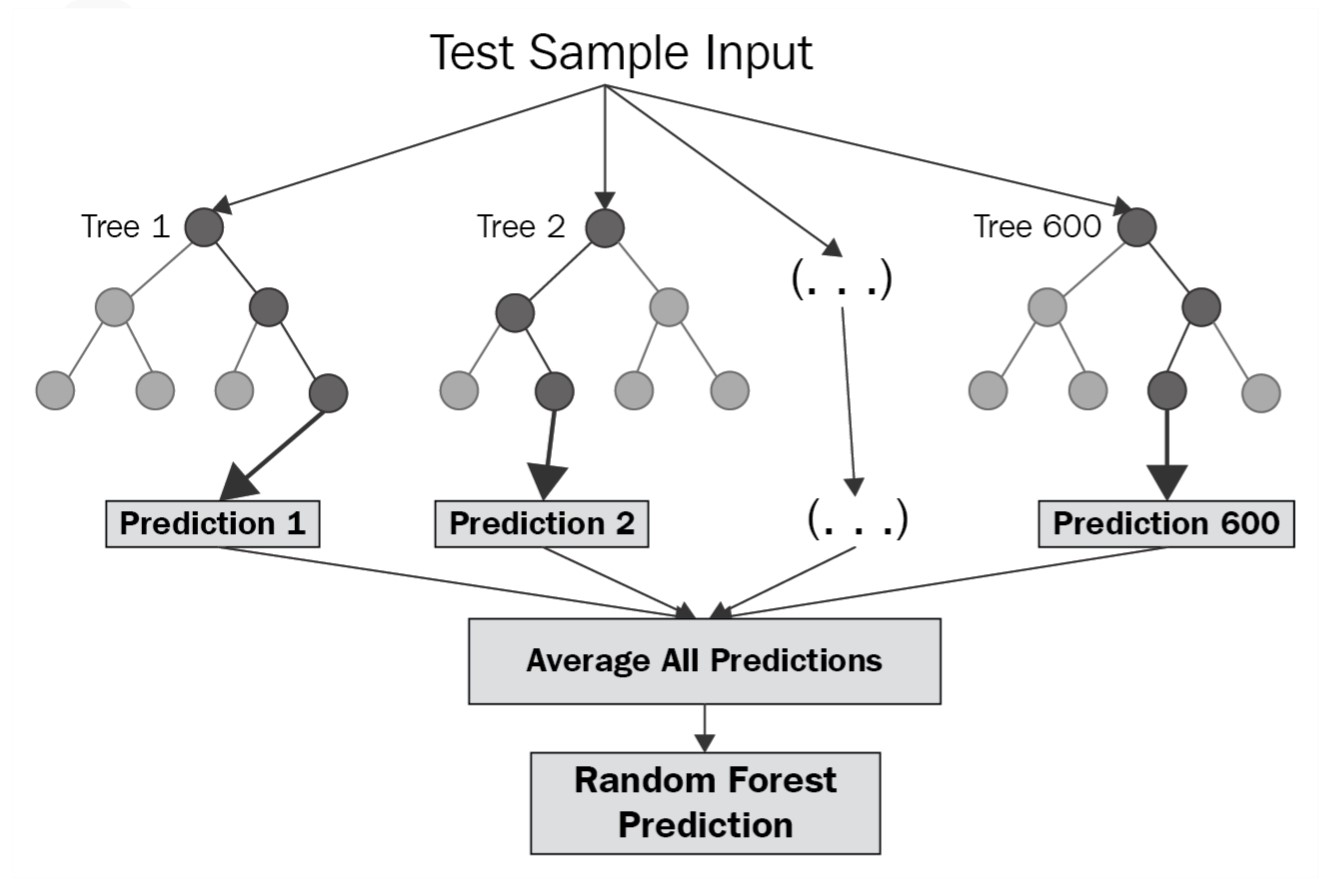
\includegraphics[scale=0.3]{img/detection/random-forest.jpg}
    \caption{Random Forest model representation}
    \label{fig:random-forest}
\end{figure}

This algorithm corrects the flaw in decision trees of overfitting the training set, i.e. overtraining a learning algorithm so much that it is only effective under very specific conditions, those of the training data.

%% HABLAR DE HIPERPARAMETROS
In our case, we have used the Random Forest algorithm of the sklearn package with a number of estimators equal to 400, as well as tuning other parameters of the model, as they have been optimised by using GridSearchCV, a tool packaged with the sklearn library that allows us to optimise hyperparameters of the model.


\begin{table}[!htp]
\centering
\begin{tabular}{|l|l|l|l|}
\hline
         & precision & recall & f1-score \\ \hline
0        & 0.81      & 0.91   & 0.86     \\ \hline
1        & 0.91      & 0.81   & 0.86     \\ \hline
accuracy & 0.86      & 100    &          \\ \hline
\end{tabular}
\caption{Statistics for Random Forest}
\label{tab:RandomForestStatistics}
\end{table}

\subsubsection{SVM}
The Support Vector Machine algorithm, also known as SVM, is used in classification and regression problems, but in our case we will focus on the former. The objective of this is to find a hyperplane that best separates two different classes of data points,\textit{ i.e.} with the widest margin between the two classes. 

This margin is defined as the maximum width of the region parallel to this hyperplane that has no interior data points. This algorithm only works on problems that allow linear separation, maximising the aforementioned margin as it can be seen in Figure~\ref{fig:SVM}.

\begin{figure}[!htp]
    \centering
    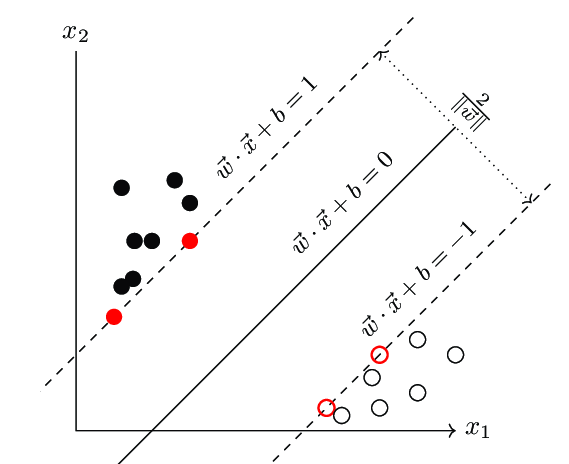
\includegraphics[scale=0.4]{img/detection/SVM.png}
    \caption{SVM model representation}
    \label{fig:SVM}
\end{figure}

%% HABLAR HIPERPARAMETROS
In our case, the configurable hyperparameters of the model have been evaluated by means of a GridSearchCV, in order to optimise it as much as possible to our data. With this, the statistics shown in table \ref{tab:SVM-statistics} have been obtained.

\begin{table}[!htp]
\centering
\begin{tabular}{|l|l|l|l|}
\hline
         & precision & recall & f1-score \\ \hline
0        & 0.78      & 0.89   & 0.83     \\ \hline
1        & 0.89      & 0.77   & 0.83     \\ \hline
accuracy & 0.83      & 100    &          \\ \hline
\end{tabular}
\caption{Statistics for SVM model}
\label{tab:SVM-statistics}
\end{table}

\subsubsection{Logistic Regression}
This model is within supervised learning and is used to predict the categorical dependent variable given a set of independent variables. This predicted output can take both categorical and discrete values and is used for classification problems. In this regression, an attempt is made to fit the values within an "S" shaped logistic function that predicts between two maximum values, either 0 or 1 as can be seen in Figure~\ref{fig:LogisticRegression}.

\begin{figure}[!htp]
    \centering
    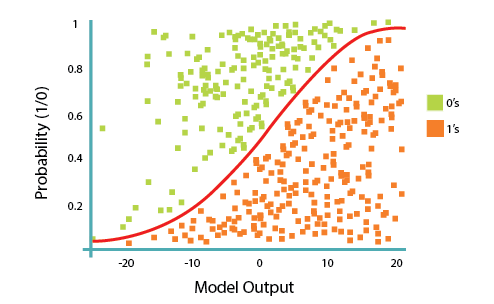
\includegraphics[scale=0.6]{img/detection/LogisticRegression.png}
    \caption{Logistic Regression representation model}
    \label{fig:LogisticRegression}
\end{figure}

Again, we proceeded to see which were the best hyperparameters for this model by using GridSearchCV, obtaining the results shown in Table~\ref{tab:LogisticRegressionStatistics}.



\begin{table}[!htp]
\centering
\begin{tabular}{|l|l|l|l|}
\hline
         & precision & recall & f1-score \\ \hline
0        & 0.80      & 0.91   & 0.85     \\ \hline
1        & 0.91      & 0.79   & 0.85     \\ \hline
accuracy & 0.85      & 100    &          \\ \hline
\end{tabular}
\caption{Statistics for Logistic Regression model}
\label{tab:LogisticRegressionStatistics}
\end{table}

\subsection{BERT Models}
After explaining the traditional models as we have called them in the present project, in which we had a mathematical algorithm that had to be trained to optimise the models to subsequently make the predictions, we are going to explain the BERT models (Bidirectional Encoder Representations from Transformers). 

BERT models are pre-trained and open source machine learning techniques based on neural networks for NLP developed by Google in 2018. These algorithms have been used in the company's search engine since 2019. BERT makes use of Transformer, an attention mechanism that learns the contextual relationships between words and includes two different mechanisms, an encoder that reads the input text and a decoder that produces a prediction. This encoder is the necessary element, because BERT's goal is to generate a language model.

BERT models can be used for a number of different linguistic tasks by adding only a small layer to the core model. In classification tasks, as is the case in this project and in sentiment analysis, they are performed in a similar way to Next Sentence Prediction (NSP), by adding a classification layer on top of the output of the token transformer (CLS).

In the NSP training process, the model is provided with pairs of sentences as input and learns whether the second sentence of the pair is the next sentence in the original document to learn about the context. 50\% of the input sentence pairs are the subsequent sentences in the original document and the other 50\% are randomly chosen and disconnected sentences. In order to process the input text the following steps are needed to be performed, as it can be seen in Figure~\ref{fig:BERTinput}.

\begin{enumerate}
    \item A CLS token and a SEP token are inserted at the beginning and end of each sentence respectively.
    \item A phrase embedding indicating phrase A or phrase B is added to each token.
    \item A positional inlay is added to each token to indicate its position in the sequence.
\end{enumerate}

\begin{figure}[!htp]
    \centering
    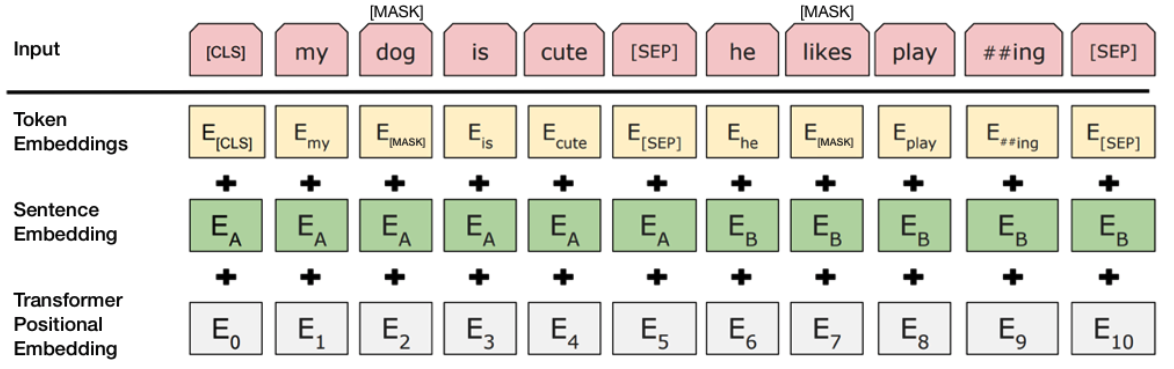
\includegraphics[scale=0.35]{img/detection/BERTinput.png}
    \caption{BERT input processing in NSP}
    \label{fig:BERTinput}
\end{figure}
Once the input text has been pre-processed, to make the prediction of the second sentence over the first, the following is needed.

\begin{enumerate}
    \item Introducing the sequence to the Transformer model.
    \item The output of the [CLS] token is transformed into a 2x1 vector using one of classification.
    \item Calculate the probability with softmax or normalised exponential function.
\end{enumerate}

BERT models, as they are pre-trained and open source, they can be packed with certain contextual representations because the model can be pretrained with different inputs. In our case, we have experimented with pure BERT implementation and two variants which are Mental roBERTa and mBERT using the Google Collab platform. We are going to discuss the results of those analysis here.

\myparagraph{BERT}
We implemented the BERT model without any specialization in its pre-training, using the bert-based-cased tokenizer and the BERTClassifier model from the Transformers library, and obtained the results shown in Table~\ref{tab:BERTstatistics}.

\begin{table}[!htp]
\centering
\begin{tabular}{|l|l|l|l|}
\hline
precision & recall & f1-score  & accuracy \\ \hline
0.566      & 0.529   & 0.495      &  0.529 \\ \hline
\end{tabular}
\caption{Statistics for BERT model}
\label{tab:BERTstatistics}
\end{table}
The results were not as good as expected so we decided to improve them by using other BERT variants pretrained with specific data that is closer to our case study.

\myparagraph{Mental roBERTa}
This model is pretrained with post related to mental health problems, which we though it would introduce an improvement in our statistics and the results we obtained were as in Table~\ref{tab:MentalroBERTastatistics}.
\begin{table}[!htp]
\centering
\begin{tabular}{|l|l|l|l|}
\hline
precision & recall & f1-score  & accuracy \\ \hline
0.737      & 0.735   &  0.735      &  0.735 \\ \hline
\end{tabular}
\caption{Statistics for Mental roBERTa model}
\label{tab:MentalroBERTastatistics}
\end{table}

As expected, results were much better using Mental roBERTa but still distant from what we achived with the other models.
\myparagraph{mBERT}
mBERT model is a regular implementation for BERT pretrained with data from more than a 100 languages, so it can provide support for multilingual applications. As it is now, our model only supports text in English but we would like to extend this functionality in the future and this is why we made test with this specific model. The obtained results are as discussed in Table~\ref{tab:mBERTstatistics}.
\begin{table}[!htp]
\centering
\begin{tabular}{|l|l|l|l|}
\hline
precision & recall & f1-score  & accuracy \\ \hline
0.651      & 0.647   & 0.647      &  0.647 \\ \hline
\end{tabular}
\caption{Statistics for mBERT model}
\label{tab:mBERTstatistics}
\end{table}

And again, as expected the model works much worse than Mental roBERTa as it is not specialized in Mental Health problems but on the other hand, we could win multilanguage support with it. \\

There are more variants that could be implemented such as patentBERT(fine-tuned to perform patent classification), bioBERT (for biomedical text mining) or SciBERT (for scientific texts), but as the results with BERT were not as good as we obtained with the traditional models, we decided to stop working but it is a field from this project that could be investigated for optimising in the future.



\subsection{Decision}
% exponer las medidas tomadas para cada modelo y dar una valoracion
As we have been reviewing, we have analysed the performance of the models Random Forest, SVM, Linear Regression and BERT (with two additional variants pretrained with specific data) and we have now the necessary criteria to make a decision on what model to choose.

So far, the model that throws the best results is \textbf{Random Forest}, which has also a small execution time, so we have decided that it will be our main model in our project. We could include mBERT as well for languages that are not English so we will review its viability as well, keeping as principal algorithm the Random Forest.

\chapter{System architecture}
% arquitectura del sistema
%API python
% web
\label{chap:architecture}

\textit{In this chapter we are going to describe a selected use case. This section will discuss the two use case: Sentiment and Emotion Analysis applying Deep Learning techniques, which will include the datasets used, the first steps with the neural networks and the use of more advance techniques.}

\clearpage

\section{General Architecture}

%This chapter will serve as a description of the methodology that has been followed in order to develop the system and meet the requirements set out in the Chapter~\ref{chap:introduction}. As mentioned, this work arises from the need of tackling a problem in today's society, namely Eating Disorders. More specifically, the aim is to help in the early detection of such illnesses so that they can be treated as soon as possible.

The aim of this project is to help in the early detection of Eating Disorders so that they can be treated as soon as possible. To achieve that, the system's presentation should be easy to handle and understandable for the people who use it. Furthermore, it has to be visually appealing in order to motivate people with a potential Eating Disorder to use it.

The presentation layer of this Master Thesis has been designed using a specific methodology based on states called bloc, which will be explained in this chapter. There are diferent parts that are part of this bloc architecture that need to be implemented in order to perform different actions that will enhance the user experience.

To serve this presentation layer with data, a server has been implemented in which an API has been constructed. The objective of this is to consult the information about the required user and predict the suffering of an Eating Disorder. This server makes calls to the Twitter API also to make the prediction using the Machine Learning model previously preloaded on the same server. The model that has been followed for implementing this part of the system is called Front Controller, which will be explained here.

The system architecture that has been developed for this Master Thesis can be seen in the Figure~\ref{fig:architecture}, where you can find the interactions between the subcomponents in a simplified diagram.

% Mostrar esquema arquitectura
\begin{figure}[h]
    \centering
    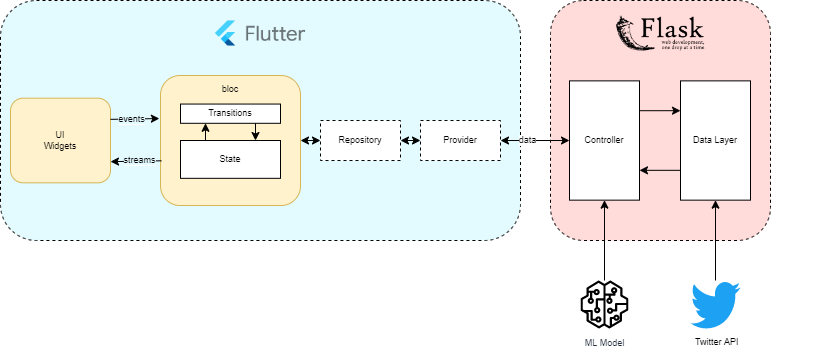
\includegraphics[width=1.05\textwidth]{img/architecture/architecture.drawio.png}
    \caption{Simplified diagram of the architecture of the system}
    \label{fig:architecture}
\end{figure}


In this figure you can see a simplified abstract diagram of the structure of our system, consisting of two distinct elements, which are the server made with Flask and the user interface for which Flutter has been used. In the following we will break down this architecture and zoom in on the different parts to explain what the elements represented in the diagram above consist of and what function they have.


\section{Flask server}
\label{sec:server}
% Funciones que realiza: Extraccion datos, procesamiento y predicción
 In this section we are going to focus on the part that obtains and processes the data from our application in order to be able to make a prediction about the user we want to analyse. The basic functions of this are data extraction, data processing and the generation of a prediction that is returned in JSON format as a response, along with additional information.
 
 We needed a technology that was fast and light as we didn't want to overcomplicate the text processing, we just wanted it to be easy to query to get the best user experience and reduce waiting times. For this reason we chose Flask, a fairly mature lightweight framework for Python, which allows us to set up a server in a matter of seconds and process requests quickly.
 
 
 
 % MODELO SEGUIDO en  arquitectura: FRONT CONTROLLER
 The model followed to implement this Flask server is the Front Controller model, which can be seen in the Figure~\ref{fig:front-controller}. This model is based on a controller that handles all requests from a server, which is useful to achieve flexibility and reuse code without redundancy.

 
\begin{figure}[h]
    \centering
    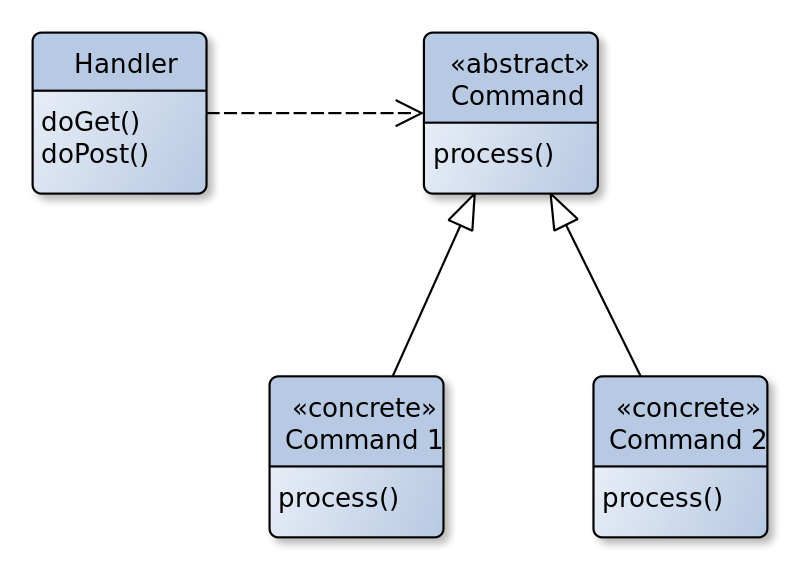
\includegraphics[width=0.65\textwidth]{img/architecture/Front_Controller.png}
    \caption{Example of Front Controller architecture}
    \label{fig:front-controller}
\end{figure}

These front controllers are normally used in web applications like the one in this project to implement flows. It serves to simplify navigation between screens and is invoked every time calls are made to the server. This Front Controller handles all the tasks common to the application, such as session, caching and in our case routing and invocation of data extraction through implemented methods.

This was the most interesting option and the one that best suited what we were looking for in this Master Thesis, as we took into account the features that we needed and the simplicity the model provides to perform and implement those features. 

The alternative would have been to have individual scripts that respond to each request, which can lead to duplication of both code and objects. Finally, this implementation was discarded because of the benefits that a front controller brings in terms of escalation and life.

The features that we required from this sever are as mentioned before, three main tasks, which are data extraction, data processing with its prediction, and data serving through the API which we will break them out in the following.

% 1. Extraccion de datos
\myparagraph{Data extraction}
The focus of this project is on the social network Twitter and because of this, we need to extract information from Twitter in order to achieve our goal. We want to analyse per user the suffering of an Eating Disorder so we need to extract the latest tweets of a specific person in order to treat them and introduce them as input to our model.

For this, we used a Python-based tool called snscrape~\cite{JustAnot83:online}, which can extract data from the Twitter API without us having to authenticate ourselves. The possibility of creating a Developer account on Twitter was considered and emails were exchanged with the administration, but it was found that there were many more complications than using this tool. 

This snscrape Python package that can be easily installed using the pip manager, allows us to take as many tweets as we want from a profile and put them in a text file in JSON format, as it can be seen in the code block described in Appendix~\ref{appendix:JSONsnscrape}.

So, it was decided to use snscrape for its simplicity and for not needing to authenticate to the API. With the command written in the Code~\ref{code:snscrape} we can access the 1000 most recent tweets of the user with the identifier \$username and save them in JSON format in the file user-tweets.json.

Subsequently, we will read this file to be able to process the information taken. The tool has more functionalities such as searching Twitter (twitter-search) or consulting a profile (twitter-profile) but this one is enough for the given approach.

\begin{lstlisting}[caption={Command executed for obtaining tweets}, label={code:snscrape}]
snscrape --jsonl --max-results 1000 twitter-user $username > user-tweets.json
\end{lstlisting}

Once we have the file ready, we read it using the pandas library in order to ingest it into our model, preprocessing it beforehand. This file is given a personal character because after reading the file, it is deleted from the server so as not to generate overload. Now, in the next paragraph, we will explain how we preprocess the text once it is read.

% 2. Procesamiento de datos (empaquetamiento de modelo) / wordcloud y prediccion
\myparagraph{Data processing and prediction}
We need to process the data obtained from twitter in our platform, so we will treat the information in a similar way in this Flask server to the one explained in~\ref{sec:preprocessing}, as we want our model to work in a similar way as it did with the validation data because it gave us good results. 


So, what we do is reuse the code written in Code~\ref{code:preprocessing} for this data extracted from Twitter. As a result we get an array of words from the last tweets published by the user in question.

%Wordcloud
In addition, we took the opportunity of having this to create more statistics and to give the user more insights. For example, we have implemented the creation of a wordcloud that reflects the most used words and their frequency in a very intuitive graphical way.

% 3. Como se sirven los datos: rutas y por JSON --> API
\myparagraph{Data serving through API}
%JSON Format and wordcloud img processing
To serve the prediction and additional statistics the API has been programmed as above. This API has a dedicated path to return the extracted results in JSON format.

The simplified output obtained by querying the API as can be seen in the Code~\ref{code:jsonapi} is a composition of the prediction result, user information and the wordcloud image in base64 format. This information is then used in the Flutter part to build the user interface.

%% METER EJEMPLO JSON
\begin{lstlisting}[caption={JSON output from API}, label={code:jsonapi}]
{
    "prediction": "0", 
    "username": "elonmusk", 
    "pic": "https://pbs.twimg.com/profile_images/1529956155937759233/Nyn1HZWF.jpg", 
    "wordcloud": "iVBORw0KGgoAAAANSUhEUgAAAZAAAADICAIAAAB..."
}
\end{lstlisting}


In order to be able to send the wordcloud image through the API, it has to be encoded in base64 format. Subsequently, it has to be decoded in the application part in order to be displayed.\\\\
In the following section we will focus on the application that the user uses, presenting its parts, the model used in its design and its structure.
\section{Flutter application}
% Presentacion de la aplicacion
The application aims to have a clear and guided user experience that engages the user for using it. It should have a clear flow for easing its manipulation and really help the person who uses it. Because of that we used Flutter for implementing it.

%Multiplataforma
It is a Flutter-based as it is mentioned, so that implies that it is a cross-platform application that can be seen in Android, iOS and web, which make it polivalent. Its content is dinamically treated so it adjusts to all kinds and sizes of screen, which has been also take into account in the design process.

% Diseño de la app: BLOC
The design pattern followed is called BloC, which makes our application based on separate components. These components contain only the business logic, \textit{i.e.} the logic that determines how information can be created, stored and changed.

BLoC is widely used in applications developed in Flutter, as it is based on widgets and BLoC helps to communicate these widgets with other components of the application.

This communication is done through the issuing of events from the UI as shown in the Figure~\ref{fig:bloc}. BLoC interprets this and transforms it into states and emits streams back to the UI to make the relevant changes to the interface. 

\begin{figure}[h]
    \centering
    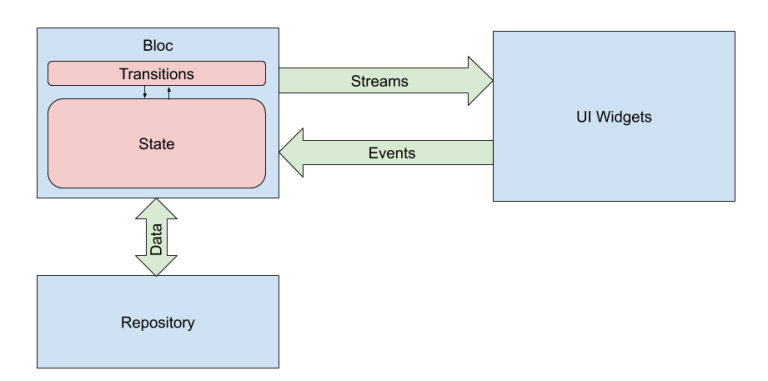
\includegraphics[width=0.85\textwidth]{img/architecture/bloc.png}
    \caption{BLoC architecture}
    \label{fig:bloc}
\end{figure}

In turn, our BLoC-based application is packed with repositories, which serve to obtain data necessary for the application, as in this case is the prediction of our system issued by the Flask server explained before. The repository of our system provides access to long-term state data, in our case via API.

% Planteamiento de la estructura general: repositories, etc

\chapter{Case study}

\label{chap:case-study}

\textit{In this chapter we are going to describe the use case of the platform, in which the reader will be guided through the displays of the system.}

\clearpage

This chapter shows the result obtained after the design and implementation of the platform. The main elements that the user encounters when navigating the platform will be shown. 

The application itself has been decided to be called \textbf{PredEating}, since it is a system that helps in the early diagnosis of Eating Disorders. Its aim is tried to be filled by predicting an outcome taking the Twitter posts of the user that is analysed. Afterwards, some other features are displayed to the user who can decide what to do.

\section{User flow}

This section will show the pages implemented in the platform as well as their parts, what can be done in them and what they are for.

\myparagraph{Landing Page}
This webpage is a simple landing that is displayed when the user access the platform, as it can be seen in Figure~\ref{fig:landing}. Here some information of the project can be seen, as well as some guidance to use the platform.


\begin{figure}[!htp]
    \centering
    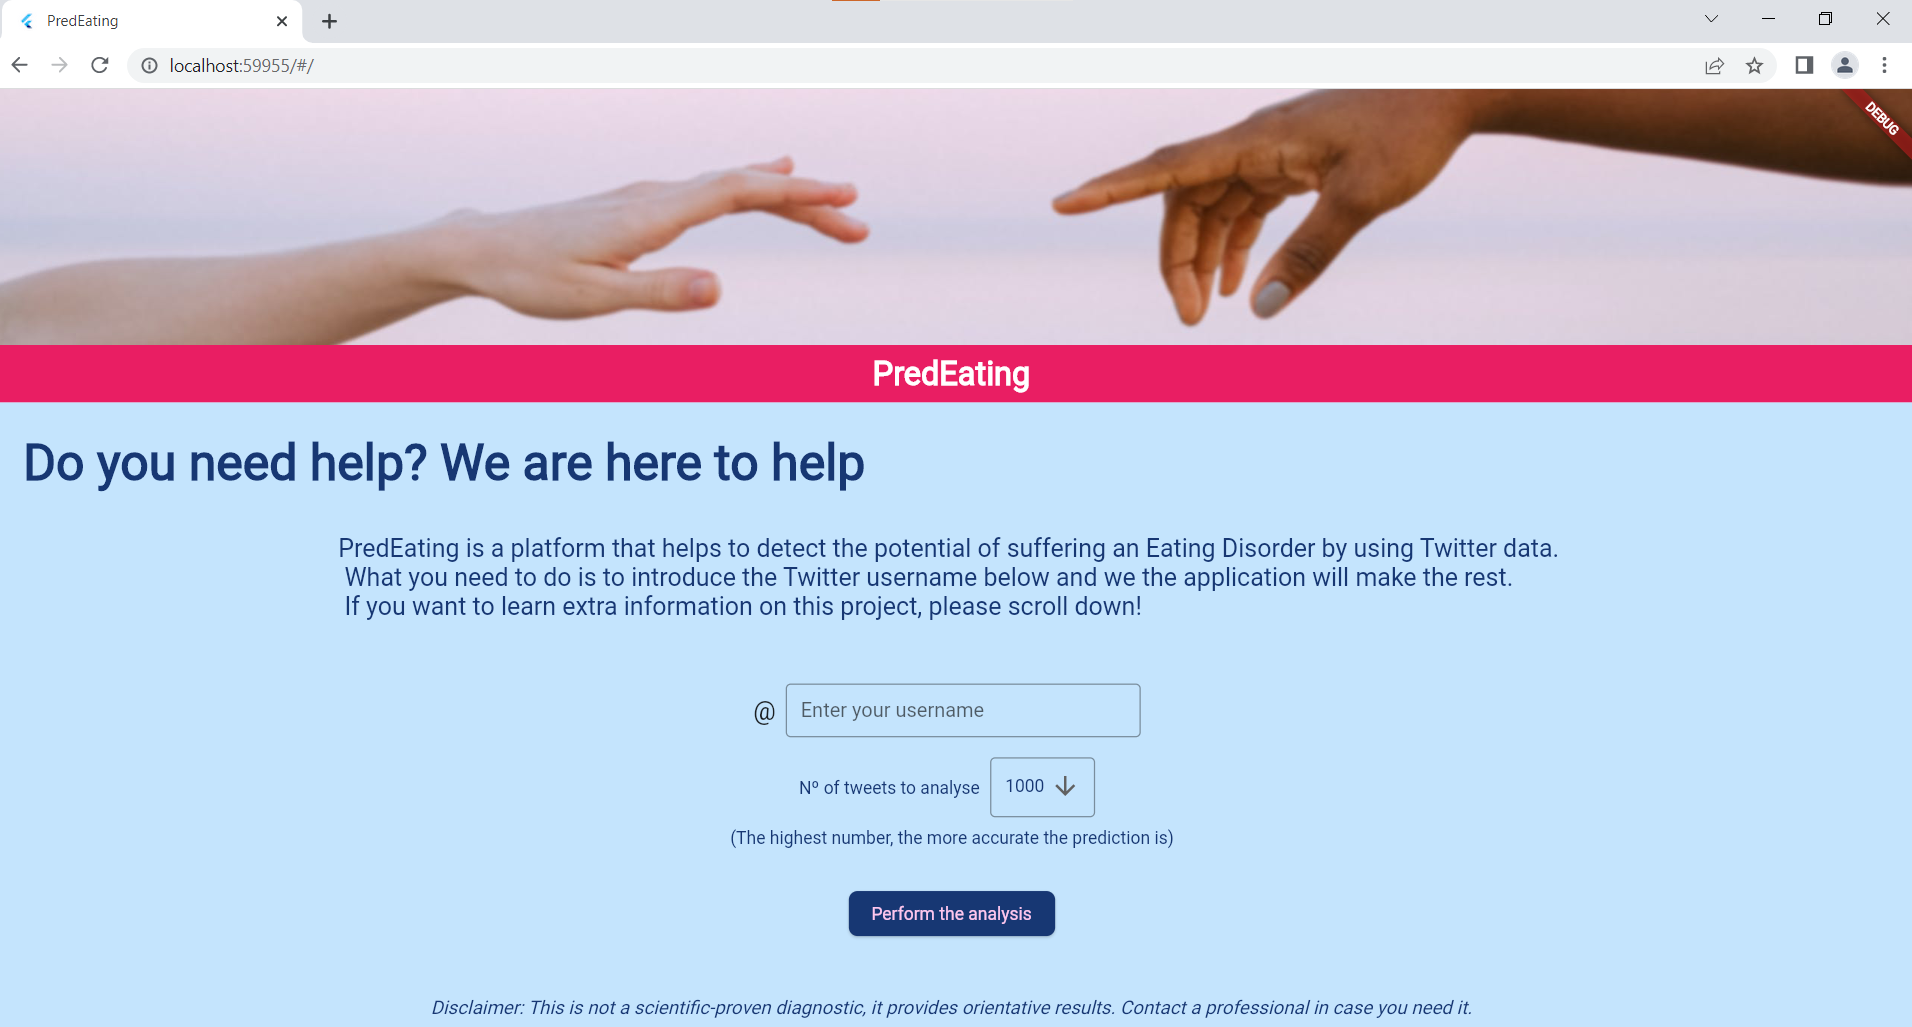
\includegraphics[scale=0.4]{img/case/landing.png}
    \caption{Landing page of PredEating}
    \label{fig:landing}
\end{figure}

As it can be seen, there is a form in the middle of the page, where the user can enter the Twitter profile to analyse. There is also another parameter which serve for modifying the number of tweets that are scrapped. If there are more, the prediction will be more accurate but on the contrary, it will take more time to process the request to the server.

There is a disclaimer because it is not a scientific-proven algorithm since it has some percentage of error. We decided to include that due to the fact that the information and the prediction are sensitive information that must be treated with a lot of responsibility.


\myparagraph{Prediction Screen}
This screen is the one which shows the results of the prediction. While the request is being processed, the page shows a loading icon and when the response from the server is received the page from the Figure~\ref{fig:predictionscreen} is shown. The sensible data has been erased because we don't want to expose any personal data.

\begin{figure}[!htp]
    \centering
    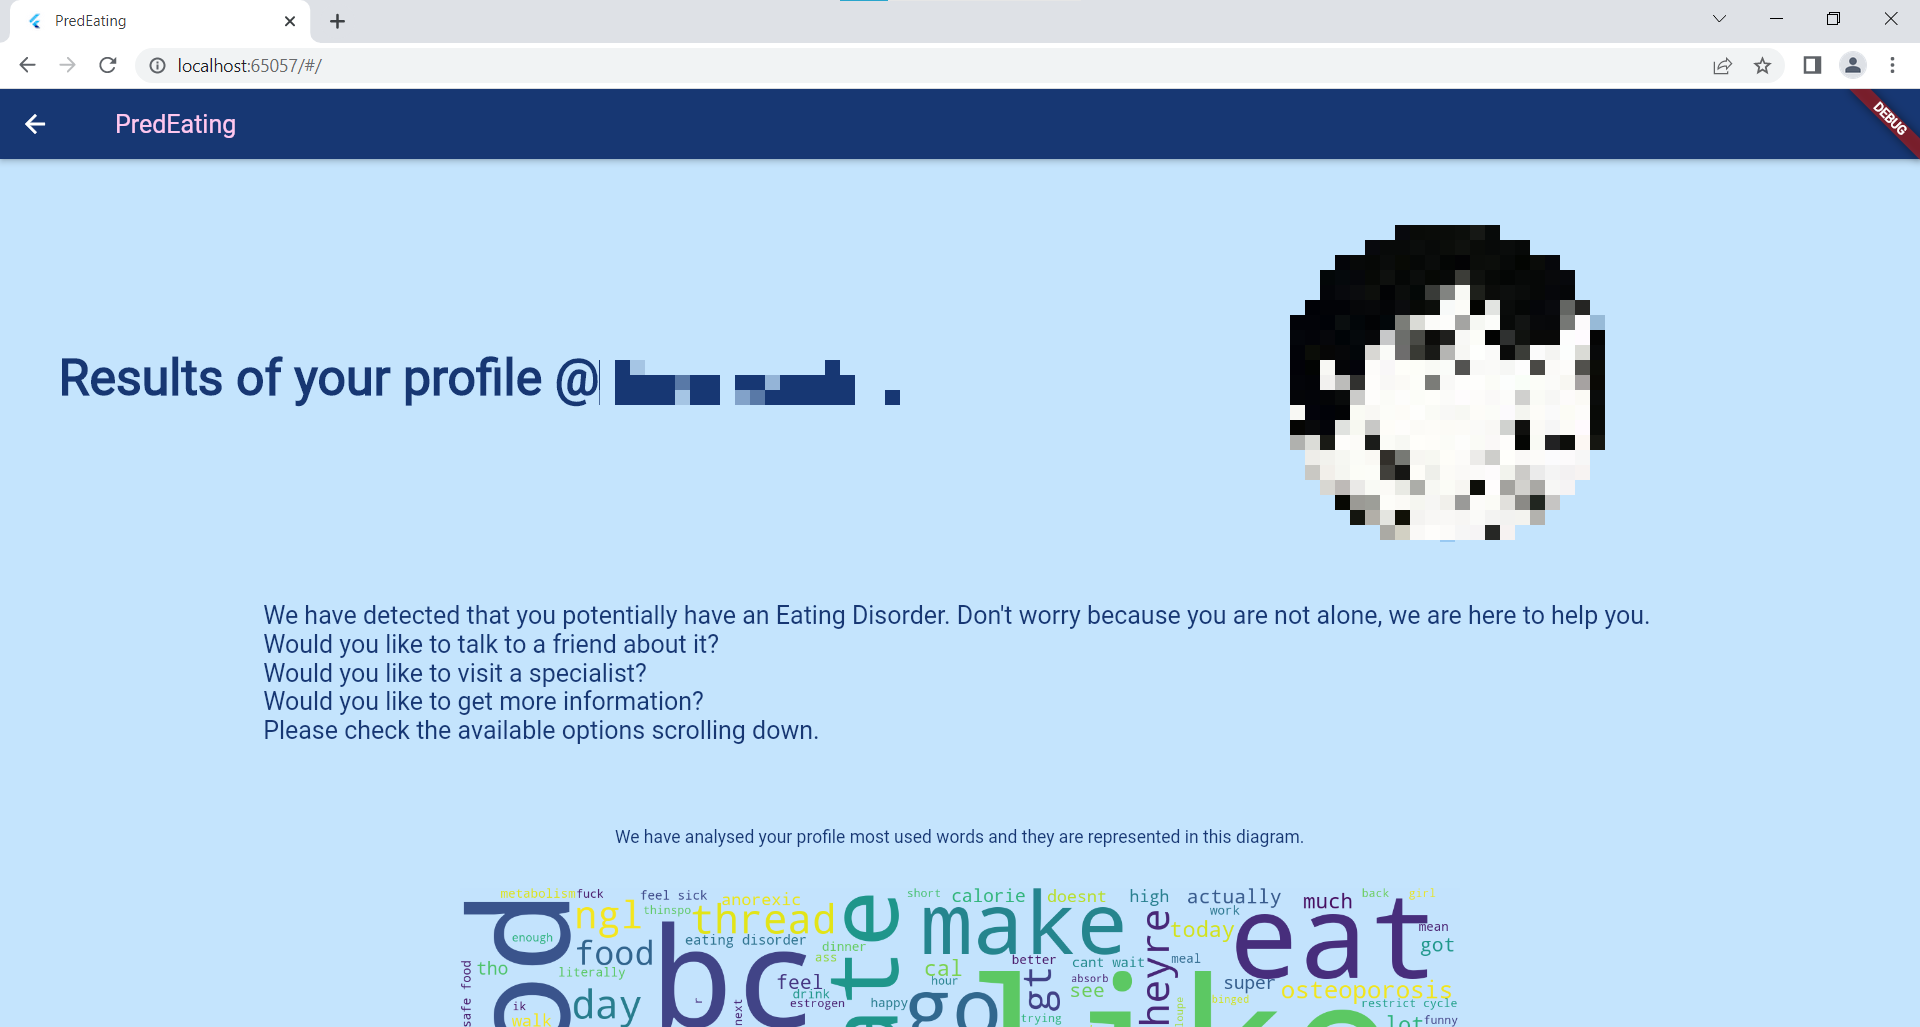
\includegraphics[scale=0.23]{img/case/predictionscreen.png}
    \caption{Prediction screen}
    \label{fig:predictionscreen}
\end{figure}

On it we can see the identifier and profile picture of the person which has been analysed. Afterwards, the prediction is shown, which can prompt either a positive prediction result or a negative one. In case of the negative, nothing else is performed on the screen.

In case the prediction is positive, we have integrated the Task Automation Service. The web server triggers an event against it when a prediction is positive. The actions that the user can take have been designed thinking on what could be useful in this situation. The possible choices the user could have are:
\begin{itemize}
    \item Contacting one of the closest friends from Twitter that the analysed user has.
    \item Contacting an organization that is focused on treating Eating Disorders.
    \item Contacting a professional for having a medical appointment.
\end{itemize}

There is also one button that can be clicked by all the users independently of the result of the prediction which serve for going to the third screen.

\myparagraph{Comparation Screen}
Here all the users could select another user profile from Twitter that can analyse and compare the most relevant information. The purpose of it is to give the user the possibility of having additional information and comparison with other users.





\chapter{Conclusions}
\label{chap:conclusions}
\textit{This chapter will describe the achieved goals done by the Master Thesis, the final conclusion and some of the key points developed in the project.}

\clearpage
\section{Achieved Goals}
A review is going to be conducted in this Chapter on what has been done and how it is matching with the objectives we posed in the Section~\ref{sec:goals}. It will revisit the key points of this project that were carried out in order to complete it.

 We have put in place the platform that we called PredEating in which users can consult the possibility of suffering an Eating Disorder. The goals that we achieved for making that possible are:
\begin{itemize}
    \item \textbf{Create and tune a Machine Learning algorithm working with NLP}. We have done several tasks in order to achieve this goal, which are detailed here.
    \begin{itemize}
        \item \textit{Data obtention and analysis}. Firstly, we got data for starting researching. A dataset specific in Mental Health diseases was found and we filtered the illnesses corresponding to Eating Disorders.
        \item \textit{Preprocessing of data}. Once we had the necessary data, we processed it in order to be able to ingest this information to our model, keeping the most relevant parts of the texts.
        \item \textit{Training and validation of Machine Learning model}. We ingested the data to different models and performed several statistical studies in order to see which one was adapting better to our data.
    \end{itemize}
    \item \textbf{Develop a web server that performs and serves the prediction}. In order to provide our system with the prediction, we needed to have a platform where we dispatch the requests. For implementing it we have performed the following tasks.
    \begin{itemize}
        \item \textit{Get data from Twitter}. We obtained the data from Twitter by scrapping the posts that a certain user have sent.
        \item \textit{Import the model for performing the prediction}. We imported the model that we have trained in the previous step for making the prediction with the Twitter data that we had scrapped.
        \item \textit{Serving of response in JSON format}. After making the prediction, we served it to the user interface by using JSON format using an API format.
        \item \textit{Providing additional information}. We sent additional information that enhances user experience together with the prediction to the user interface.
    \end{itemize}
    \item \textbf{Design and implement an easy-to-use user interface}. We have implemented a cross-platform application in which the user can analyse Twitter profiles. They can interact with the system and get more statistics if they want to. If the prediction is positive, some actions have been implemented based on the automation platform.
    \item \textbf{Integrate our platform with an external system for automatising processes}. We provided an enhanced user experience by using automatic tasks that are triggered once the prediction with a positive result is received.
\end{itemize}

\section{Conclusion}
\label{sec:conclusion}

To begin with, the main objective of this project was to \textbf{develop a system for the analysis and detection of Eating Disorder-related mental health problems in social networks}.

This objective has been achieved following the steps detailed in the previous subsection, which recapitulate the goals marked in the Section~\ref{sec:goals}. Data has been obtained for training and optimising a Machine Learning model. This model has been exported into a web server which perform actions on scrapped Twitter data dispatches the results as a API response. The user interface interprets this response for showing the prediction to the user, bringing also some facilities in case it is positive. The integration that we have implemented opens a wide variety of possibilities in which the platform can develop into. 

We can conclude that this platform has potential to help patients in the earliest stages of the disease. It should be tested in real cases but for now, it can be considered as a potential improvement in the sanity process if it is finally deployed into a production environment. We have also seen the importance of social networks, both for getting data and for exploring how users are interacting with it. These can be exploited to construct beneficial applications for the society and its good.


\section{Future work}
The PredEating platform has been implemented but as the machine learning field is that big and changeable, there is always room for improvement. In our case, there are some actions that can be beneficial to the system if they are studied and implemented.
\begin{itemize}
    \item \textbf{Dataset variation}. Models and do the processing needs to be done with other data to give versatility and reliability to our Machine Learning model. With this the prediction could be improved and it will give more perspective to the learning.
    \item \textbf{Better optimisation of BERT models}. A simple analysis of BERT models has been made. Due to their complexity, there are many parameters that can be optimised using different configurations to look for synergies between them. For the future it is an improvement that could be made as these models usually give better results than the ones obtained in this Master Thesis.
    \item \textbf{Discern between Eating Disorders}. Another improvement that can be implemented in this project is to train the Machine Learning algorithm to develop the ability to differentiate between the different Eating Disorders that are present in society.
    \item \textbf{User experience features}. A simplistic, result-oriented approach to the application has been followed, although this application can be improved by including features that are useful to the user. These new features can range from being able to integrate new automations to including new screens and navigation modes in the user interface.
\end{itemize}




% apendices del proyecto
\appendix
\chapter{JSON from snscrape}
\label{appendix:JSONsnscrape}

The JSON that is coming from the scrapping tool snscrape has the following structure.

\begin{lstlisting}[label={code:JSONtweets}, caption={JSON output from snscrape}]
{
    "_type": "snscrape.modules.twitter.Tweet", 
    "url": "https://twitter.com/machinelearnflx/status/1536005123603824641", 
    "date": "2022-06-12T15:18:53+00:00", 
    "content": "The best books about machine learning for beginners https://t.co/iO29u5OHzb  #MachineLearning", "renderedContent": "The best books about machine learning for beginners shepherd.com/best-books/mac\u2026  #MachineLearning", 
    "id": 1536005123603824641, 
    "user": {"_type": "snscrape.modules.twitter.User", 
            "username": "machinelearnflx", 
            "id": 4820804277, 
            "displayname": "Machine Learning", 
            "description": "Everything about #MachineLearning, #DeepLearning  #AI  #Bigdata  #Analytics #DataMining, #DataScience #Courses #Learning linktr.ee/machinelearnflx", "rawDescription": "Everything about #MachineLearning, #DeepLearning  #AI  #Bigdata  #Analytics #DataMining, #DataScience #Courses #Learning https://t.co/9yIo7fVa7l", "descriptionUrls": [{"text": "linktr.ee/machinelearnflx", 
                                "url": "https://linktr.ee/machinelearnflx", 
                                "tcourl": "https://t.co/9yIo7fVa7l", 
                                "indices": [121, 144]}], 
            "verified": false, 
            "created": "2016-01-17T11:55:58+00:00", 
            "followersCount": 132067, 
            "friendsCount": 36853,
            "statusesCount": 488349, 
            "favouritesCount": 220, 
            "listedCount": 2655, 
            "mediaCount": 11, 
            "location": "", 
            "protected": false, "
            linkUrl": "https://linktr.ee/machinelearnflx", "
            linkTcourl": "https://t.co/9yIo7fVa7l", 
            "profileImageUrl": "https://pbs.twimg.com/profile_images/688735459892195329/v8sHaWSG_normal.jpg", 
            "profileBannerUrl": "https://pbs.twimg.com/profile_banners/4820804277/1504968657", 
            "label": null, 
            "url": "https://twitter.com/machinelearnflx"}, 
    "replyCount": 0, 
    "retweetCount": 1, 
    "likeCount": 5, 
    "quoteCount": 0, 
    "conversationId": 1536005123603824641, 
    "lang": "en", 
    "source": "<a href=\"https://twitter.com/pythonbot_\" rel=\"nofollow\">Postmatico</a>", 
    "sourceUrl": "https://twitter.com/pythonbot_", 
    "sourceLabel": "Postmatico", 
    "outlinks": ["https://shepherd.com/best-books/machine-learning-for-beginners"], 
    "tcooutlinks": ["https://t.co/iO29u5OHzb"], 
    "media": null, 
    "retweetedTweet": null, 
    "quotedTweet": null, 
    "inReplyToTweetId": null, 
    "inReplyToUser": null, 
    "mentionedUsers": null, 
    "coordinates": null, 
    "place": null, 
    "hashtags": ["MachineLearning"], 
    "cashtags": null
}

\end{lstlisting}
\chapter{Social, economic, environmental and ethical aspects}

In this section we will analyse the social, economic, environmental an ethical impact of this Master Thesis.

\section{Introduction}
Today's technologies allow universal access to research resources, so this work can be consulted anywhere in the world as it can be found on the department's website, having a global impact.

The development of this project provides a contribution that not only affects the area of research and in this particular case research in Telecommunications. It also affects the area of health in which this project is framed, as it has been developed and will be exposed in a public way.


\section*{Social impact}
This work focuses on the health framework, specifically on mental health and Eating Disorders, affecting people related to this topic. This project intends to provide help for the early detection of these pathologies in order to accelerate the diagnostic process without the intention of substituting anything already established.

With this, it is intended to reinforce healthcare in early detection, as it is the most key and critical step in the process. The patient's recovery time and the extent of the disease depends on optimising it.

\section{Economic impact}
Regarding the economic impact, this project doesn't have a huge economic implication other than the cost it could save in the long run if the disease is treated before and takes less recovering time for the patient. The distribution is thought to be open and public so there won't be any direct economical repercussion.

We wanted to discuss the possibility that this project enables by social media mining. It can save costs and time compared to traditional approaches, which can be taken up by companies and public institutions. These institutions are usually the ones that carry studies related to health, so they could be the major beneficiary of this present project.

\section{Environmental impact}

Technology has always an impact in nature undoubtedly. This is called ecological footprint which can be define as the quantity of nature it takes to support people or economy. Considering the nature of this project, it can be assured that it does not have a notable environmental impact, as the only resources used are the electronic equipment and the electricity that supplies it, these resources being very limited.

\section{Ethical and professional responsibility}

This Master Thesis uses Twitter, which could incur into an ethical discussion. We use tweets of users together with the user names. In Twitter's privacy policy, it is public and tweets can be viewed and searched. We only use the tweets from public accounts which owners have not restricted them. It implies that it is public that and it is usable.

Also, this project tackles information which is really sensible and requires a lot of awareness and consciousness on what is been treated. This is why we have left the system with disclaimers and comments that this is not a scientific-proven platform rather a support and helper for the medical system.

\section{Conclusions}

This project will help potential users suffering from an Eating Disorder to consult a prediction of their approximate profile. They are encouraged to take the next step to be treated if they are positive, in order to improve and treat the illness appropriately with a dedicated organisation or a medical specialist. It is the germ of a great concept, as it has great potential, which is expected to be exploited in the near future.

\chapter{Budget}
\label{sec:budget}


The budget elaborated for this project consists of the following items.
\begin{itemize}
    \item Material execution budget
        \begin{itemize}
            \item Material resources budget
            \item Labour costs
        \end{itemize}
    \item Total project costs
    \item Overheads and industrial profit
    \item Total budget
\end{itemize}

\section*{Material execution budget}
The material execution budget together with the overheads and the industrial profit constitute what is called the contract execution budget, which is referred to as the total budget.

All budgets shall be presented in Euros (\euro).

\subsection*{Material resources budget}

Next, in the Table~\ref{tab:hardware}, we find the material resources used throughout the project.

\begin{table}[]
\centering
\begin{tabular}{|lrr|r|}
\hline
\multicolumn{1}{|c|}{\textbf{Concept}} & \multicolumn{1}{c|}{\textbf{Cost}} & \multicolumn{1}{c|}{\textbf{Amortisation}} & \multicolumn{1}{c|}{\textbf{Real cost}} \\ \hline
\multicolumn{1}{|l|}{Principal laptop} & \multicolumn{1}{r|}{1.945,10}      & 16.66\%                                    & 324.05                                  \\ \hline
\multicolumn{1}{|l|}{Server PC}        & \multicolumn{1}{r|}{820,00}        & 16.66\%                                    & 136,37                                  \\ \hline
\multicolumn{1}{|l|}{Screen}           & \multicolumn{1}{r|}{531,19}        & 16.66\%                                    & 88.5                                    \\ \hline
\multicolumn{1}{|l|}{Keyboard}         & \multicolumn{1}{r|}{15}            & 16.66\%                                    & 2.5                                     \\ \hline
\multicolumn{1}{|l|}{Mouse}            & \multicolumn{1}{r|}{15}            & 16.66\%                                    & 2.5                                     \\ \hline\hline
\multicolumn{3}{|l|}{\textbf{Total cost}}                                                                                         & \textbf{553.92}                         \\ \hline
\end{tabular}
\caption{Material resources budget}
\label{tab:hardware}
\end{table}

\subsection*{Labour costs}
The project required the participation of an engineer who implemented the system and put it into operation. This profile falls within contribution group 1 of the General Social Security Scheme, with a working day of 8 hours a day and 21 days a month. The complete breakdown can be consulted in the Table~\ref{tab:labour}.

\begin{table}[h]
\centering
\begin{tabular}{|lcc|r|}
\hline
\multicolumn{1}{|c|}{\textbf{Position}} & \multicolumn{1}{c|}{\textbf{Hours}} & \textbf{Price/Hour}     & \multicolumn{1}{c|}{\textbf{Total}} \\ \hline
\multicolumn{1}{|l|}{Engineer}          & \multicolumn{1}{r|}{1050}           & \multicolumn{1}{r|}{16} & 16800                               \\ \hline\hline
\multicolumn{3}{|l|}{\textbf{Total cost}}                                                                        & \textbf{16800}                      \\ \hline
\end{tabular}
\caption{Labour Costs}
\label{tab:labour}
\end{table}


\subsection*{Total resources cost}
The total cost of resources is made up of the cost of material resources and labour. Its breakdown can be seen in the Table~\ref{tab:totalresources}.

\begin{table}[]
\centering
\begin{tabular}{|l|r|}
\hline
\multicolumn{1}{|c|}{\textbf{Concept}} & \multicolumn{1}{c|}{\textbf{Cost}} \\ \hline
Material resources                     & 16800                              \\ \hline
Labor                                  & 553.92                             \\ \hline\hline
\textbf{Total cost}                    & \textbf{17353.92}                  \\ \hline
\end{tabular}
\caption{Total resources costs}
\label{tab:totalresources}
\end{table}

\section*{Overheads and industrial profit}
Under the chapter of general expenses are included all those indirect expenses derived from the use of installations, depreciations, fiscal expenses, etc. With this, the execution budget by contract is as shown in the Table~\ref{tab:overheads}.

\begin{table}[h]
\centering
\begin{tabular}{|l|r|}
\hline
\multicolumn{1}{|c|}{\textbf{Concept}}        & \multicolumn{1}{c|}{\textbf{Cost}} \\ \hline
Material Execution Budget                     & 17353.92                           \\ \hline
Overheads (16\% of MEB)                       & 2776.63                            \\ \hline
Industrial profit (6\% of MEB)                & 1041.23       \\ \hline\hline
\textbf{Total contract implementation budget} & \textbf{21171.78}                  \\ \hline
\end{tabular}
\caption{Overheads and industrial profit}
\label{tab:overheads}
\end{table}

\section*{Total Budget}
Applying 21\% Value Added Tax (VAT), the total budget shown in the table below is obtained. the Table~\ref{tab:total}. The total budget of the project amounts twenty-five thousand six hundred and seventeen and eighty-five cents.

\begin{table}[h]
\centering
\begin{tabular}{|l|r|}
\hline
\multicolumn{1}{|c|}{\textbf{Concept}} & \multicolumn{1}{c|}{\textbf{Cost}} \\ \hline
Budget subtotal                        & 21171.78                           \\ \hline
VAT (21\%)                             & 4446.07                            \\ \hline
\textbf{Total budget}                  & \textbf{25617.85}                  \\ \hline
\end{tabular}
\caption{Total budget}
\label{tab:total}
\end{table}

\begin{flushright}
  Madrid, 23rd June 2022\\
  \rule{0pt}{2cm}

  Javier Antón Yuste\\
\end{flushright}

\phantomsection
\nocite{*}
\addcontentsline{toc}{chapter}{Bibliography}
%ieeetr
\bibliographystyle{plain}
{
\small
\bibliography{biblio/ref}
}

%\cleardoublepage
\end{document}